\documentclass[runningheads]{llncs}



\usepackage{enumitem}


\usepackage{color}

\usepackage{graphicx}
\usepackage{tikz}
\usepackage{calc}
\usepackage{array}

\usepackage{amsmath, amssymb}
\DeclareMathOperator*{\argmin}{arg\,min}

\usepackage{graphbox}
\usepackage{wasysym}

\usetikzlibrary{automata,arrows}

\usepackage{comment}

\usepackage{wrapfig}


\title{On the power of oritatami cotranscriptional folding with unary bead sequence\thanks{This work is supported in part by KAKENHI Grant-in-Aid for Challenging Research (Exploratory) No.~18K19779 granted to S.~Z.~F. and S.~S. and JST Program to Disseminate Tenure Tracking System No.~6F36 granted to S.~S.}
}
\titlerunning{Power of unary oritatami cotranscriptional folding}
\author{
Szil\'{a}rd Zsolt Fazekas\inst{1} \and 
Kohei Maruyama\thanks{Primary corresponding author (\email{k.maruyama@uec.ac.jp})} \and
Reoto Morita \and \\
Shinnosuke Seki\inst{2}\thanks{Secondary corresponding author (\email{s.seki@uec.ac.jp})}
}
\institute{
Akita University, 
Graduate School of Engineering Science, 
1-1 Tegate Gakuen-machi, Akita, 0108502, Japan \\
%\email{szilard.fazekas@ie.akita-u.ac.jp}
\and
The University of Electro-Communications, 
Graduate School of Informatics and Engineering, 
1-5-1 Chofugaoka, Chofu, Tokyo, 1828585, Japan \\
}

\begin{document}

\maketitle

\begin{abstract}
We investigate simple oritatami systems in an attempt to establish lower bounds on the size and complexity of computationally universal systems. 
In particular, we look at oritatami systems, where the folding sequence consists of a number of beads of the same type and show that under reasonable assumptions, these systems are not universal.
\end{abstract}

%------------------------------------------------------
	\section{Introduction}
%------------------------------------------------------

\begin{figure}[htb]
\centering
\begin{minipage}{0.6\linewidth}
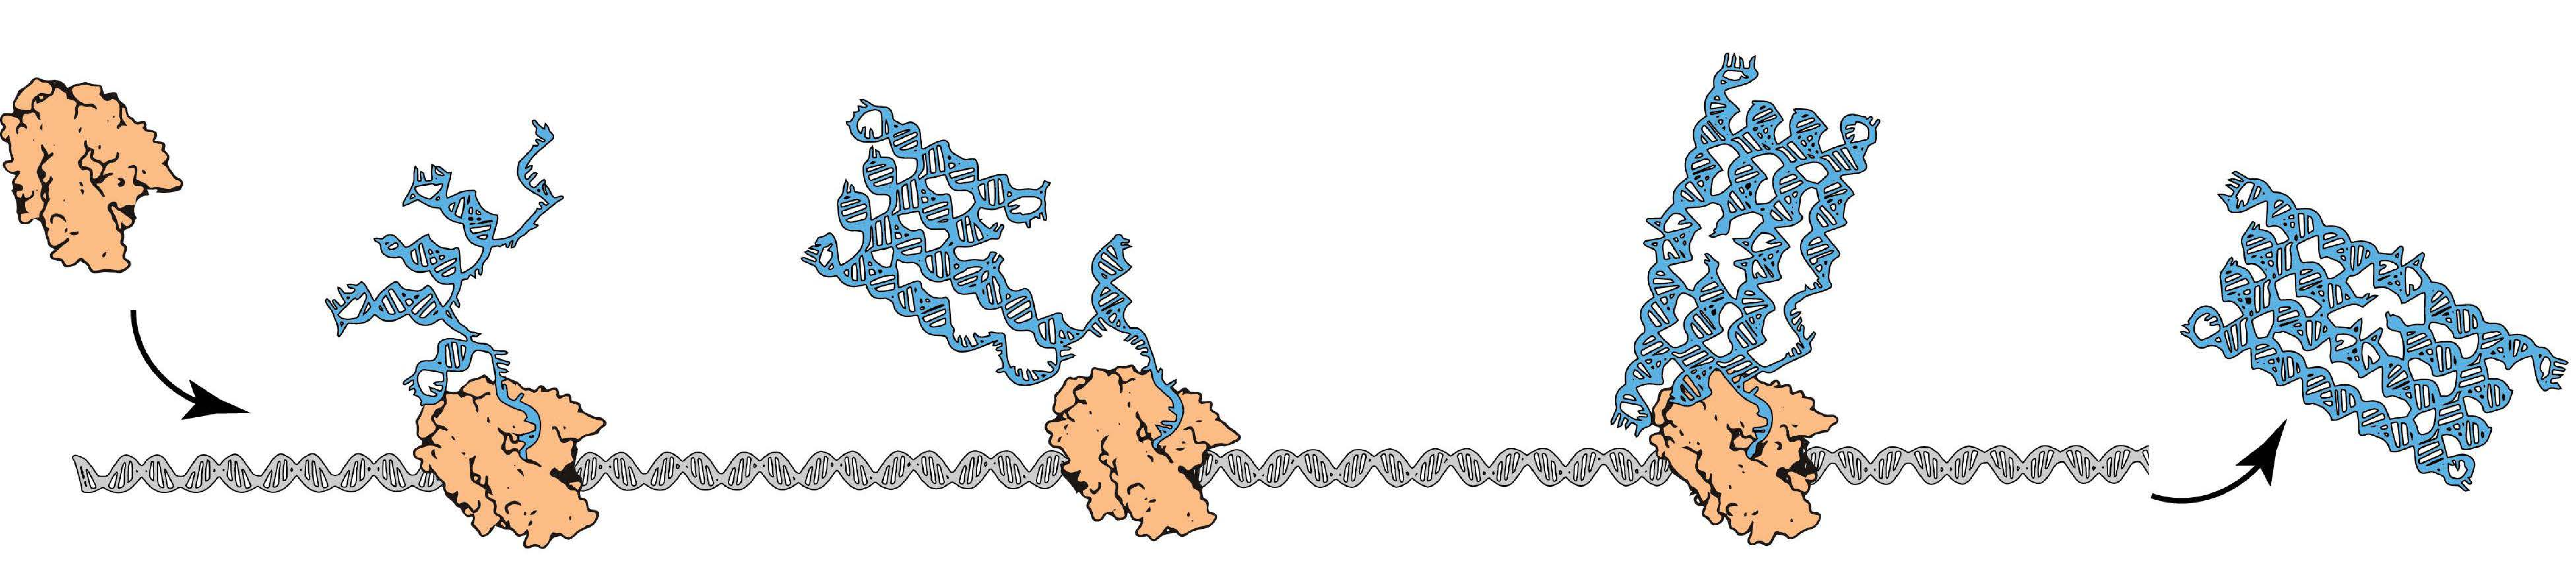
\includegraphics[width=\linewidth]{Fig/rna_origami.pdf}
\end{minipage}
\begin{minipage}{0.05\linewidth}
\centering
{\Large $\Rightarrow$}
\end{minipage}
\begin{minipage}{0.3\linewidth}
\scalebox{0.3}{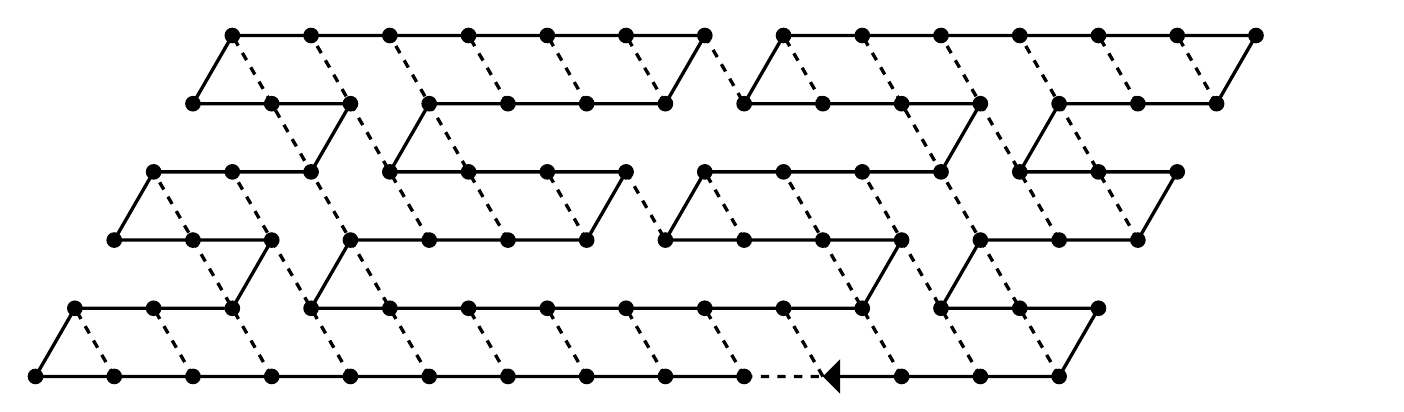
\begin{tikzpicture}
\tikzstyle{mol} = [fill,circle,inner sep=2pt]

\draw[-triangle 90, very thick] (3, 0) node[mol] {}
-- ++(180:1) node[mol] {}
-- ++(180:1) node[mol] {}
-- ++(180:1) node[mol] {}
-- ++(180:1) node[mol] {}
-- ++(180:1) node[mol] {}
-- ++(180:1) node[mol] {}
-- ++(180:1) node[mol] {}
-- ++(180:1) node[mol] {}
-- ++(180:1) node[mol] {}
-- ++(60:1) node[mol] {}
-- ++(0:1) node[mol] {}
-- ++(0:1) node[mol] {}
-- ++(60:1) node[mol] {}
-- ++(180:1) node[mol] {}
-- ++(180:1) node[mol] {}
-- ++(60:1) node[mol] {}
-- ++(0:1) node[mol] {}
-- ++(0:1) node[mol] {}
-- ++(60:1) node[mol] {}
-- ++(180:1) node[mol] {}
-- ++(180:1) node[mol] {}
-- ++(60:1) node[mol] {}
-- ++(0:1) node[mol] {}
-- ++(0:1) node[mol] {}
-- ++(0:1) node[mol] {}
-- ++(0:1) node[mol] {}
-- ++(0:1) node[mol] {}
-- ++(0:1) node[mol] {}
-- ++(240:1) node[mol] {}
-- ++(180:1) node[mol] {}
-- ++(180:1) node[mol] {}
-- ++(180:1) node[mol] {}
-- ++(240:1) node[mol] {}
-- ++(0:1) node[mol] {}
-- ++(0:1) node[mol] {}
-- ++(0:1) node[mol] {}
-- ++(240:1) node[mol] {}
-- ++(180:1) node[mol] {}
-- ++(180:1) node[mol] {}
-- ++(180:1) node[mol] {}
-- ++(240:1) node[mol] {}
-- ++(0:1) node[mol] {}
-- ++(0:1) node[mol] {}
-- ++(0:1) node[mol] {}
-- ++(0:1) node[mol] {}
-- ++(0:1) node[mol] {}
-- ++(0:1) node[mol] {}
-- ++(0:1) node[mol] {}
-- ++(60:1) node[mol] {}
-- ++(180:1) node[mol] {}
-- ++(180:1) node[mol] {}
-- ++(180:1) node[mol] {}
-- ++(60:1) node[mol] {}
-- ++(0:1) node[mol] {}
-- ++(0:1) node[mol] {}
-- ++(0:1) node[mol] {}
-- ++(60:1) node[mol] {}
-- ++(180:1) node[mol] {}
-- ++(180:1) node[mol] {}
-- ++(180:1) node[mol] {}
-- ++(60:1) node[mol] {}
-- ++(0:1) node[mol] {}
-- ++(0:1) node[mol] {}
-- ++(0:1) node[mol] {}
-- ++(0:1) node[mol] {}
-- ++(0:1) node[mol] {}
-- ++(0:1) node[mol] {}
-- ++(240:1) node[mol] {}
-- ++(180:1) node[mol] {}
-- ++(180:1) node[mol] {}
-- ++(240:1) node[mol] {}
-- ++(0:1) node[mol] {}
-- ++(0:1) node[mol] {}
-- ++(240:1) node[mol] {}
-- ++(180:1) node[mol] {}
-- ++(180:1) node[mol] {}
-- ++(240:1) node[mol] {}
-- ++(0:1) node[mol] {}
-- ++(0:1) node[mol] {}
-- ++(240:1) node[mol] {}
-- ++(180:1) node[mol] {}
-- ++(180:1) node[mol] {}
-- ++(180:1)
;

\draw[dashed, very thick]
(-5, 0) -- ++(120:1)
(-4, 0) -- ++(120:1)
(-3, 0) -- ++(120:3)
(-2, 0) -- ++(120:3)
(-1, 0) -- ++(120:5)
(0, 0) -- ++(120:1) ++(120:1) -- ++(120:3)
(1, 0) -- ++(120:1) ++(120:1) -- ++(120:3)
(2, 0) -- ++(120:1) ++(120:1) -- ++(120:1) ++(120:1) -- ++(120:1)
(3, 0) -- ++(120:1) ++(120:3) -- ++(120:1)
(4, 0) -- ++(120:1) ++(120:1) -- ++(120:1) ++(120:1) -- ++(120:1)
(5, 0) -- ++(120:3)
(6, 0) -- ++(120:3) ++(120:1) -- ++(120:1)
(7, 0) -- ++(120:5)
(8, 0) ++(120:2) -- ++(120:3)
(9, 0) ++(120:2) -- ++(120:3)
(10, 0) ++(120:4) -- ++(120:1)
(11, 0) ++(120:4) -- ++(120:1)
(3, 0) -- ++(0:1)
;

\foreach \y in {3, 5} {
\draw[dashed,very thick] (0, 0)++(60:\y) -- ++(300:1);	
}

\end{tikzpicture}}

\end{minipage}
\caption{
(Left) RNA origami. 
(Right) an abstraction of its product, i.e., an RNA tile, as a configuration of an oritatami system. A dot $\bullet$ in the figure on the right represents a sequence of 3-4 nucleotides, and the solid arrow and dashed lines represent its RNA transcript and interactions (respectively) based on hydrogen bonds between nucleotides.
}
\label{fig:rna_origami}
\end{figure}

Transcription is the first essential step of gene expression, in which a DNA template sequence is copied into a single stranded RNA sequence by a `molecular Xerox' called RNA polymerase, letter by letter according to the complimentarity relation ${\tt A} \rightarrow {\tt U}$, ${\tt G} \rightarrow {\tt C}$, ${\tt C} \rightarrow {\tt G}$, and ${\tt T} \rightarrow {\tt A}$. 
The copied RNA sequence is called \textit{transcript}. 
The transcript starts folding upon itself into intricate structures immediately after it emerges from the polymerase, as illustrated in Fig.~\ref{fig:rna_origami} (Left). 



In a recent breakthrough in molecular engineering by Geary, Rothemund and Andersen~\cite{GearyRothemundAndersen2014} the co-transcriptional folding of RNA is controlled by careful design of the DNA template. As demonstrated in laboratory, this method, called RNA Origami, makes it possible to cotranscriptionally self-assemble a unique RNA rectangular tile highly probably (see Fig.~\ref{fig:rna_origami} (Left)). 
Geary et al.~\cite{GeMeScSe2016} proposed a mathematical model for this process, called oritatami system. 
In this model, an RNA structure is abstracted as a directed path with information on hydrogen-based interaction (bonds) over the triangular grid graph $\mathbb{T}$ as illustrated in Fig.~\ref{fig:rna_origami}. 
An oritatami system folds a transcript of abstract molecules (beads) of finite number of types over $\mathbb{T}$. 
This model has been just proved efficiently Turing universal in \cite{GeMeScSe2018} by simulating cyclic tag systems introduced by Cook~\cite{Cook2004}. 
The simulation involves a very large and complex oritatami system. 
This system is deterministic in the sense that every bead is stabilized uniquely point-wise as well as interaction-wise (for the formal definition, see Sect.~\ref{sec:preliminaries}). 
One future direction of research is to quest for a smaller Turing-universal oritatami system.




Closely related is the question of where not to look for universal systems, i.e., what are the limitations of simple oritatami system. 
In search for simple oritatami systems, there are a number of restrictions one can pose on them:
\begin{itemize}
\item bounds on the relative speed of transcription to folding (delay), the number of bead types, or the number of hydrogen bonds per bead (arity);
\item bounds on the length of the transcript or on the complexity of rules to decide what types of beads interact with each other (attraction rules);
\item structural conditions on the transcript or the attraction rules.
\end{itemize}
%
In \cite{DHOPRSST2018}, Demaine et al. proved that at delay 1 and arity 1, upon an initial structure of $n$ beads, a deterministic oritatami system cannot fold into any conformation of more than $10n$ beads, no matter how many bead types are available. 
We consider this finiteness problem for unary oritatami systems under various settings of the values of delay and arity, which is formalized as follows. 

\begin{problem}\label{prob:det_unary_length}
Give an upper bound on the length of a transcript of a delay-$\delta$, arity-$\alpha$ deterministic unary oritatami system whose seed is of length $n$ by a function in $\delta$, $\alpha$, and $n$. 
\end{problem}

\begin{figure}[tb]
  \begin{center}
    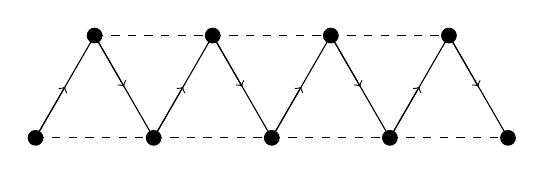
\begin{tikzpicture}
      \fill (0,0) circle[radius = 0.1];
      \fill (1.5,0) circle[radius = 0.1];
      \fill (3,0) circle[radius = 0.1];
      \fill (4.5,0) circle[radius = 0.1];
      \fill (6,0) circle[radius = 0.1];

      \draw[dashed] (0,0)--(1.5,0);
      \draw[dashed] (1.5,0)--(3,0);
      \draw[dashed] (3,0)--(4.5,0);
      \draw[dashed] (4.5,0)--(6,0);
      \draw[->] (0,0)--(60:0.75);
      \draw[->] (1.5,0)--++(60:0.75);
      \draw[->] (3,0)--++(60:0.75);
      \draw[->] (4.5,0)--++(60:0.75);
      \draw (0,0)--(60:1.5);
      \draw (1.5,0)--++(60:1.5);
      \draw (3,0)--++(60:1.5);
      \draw (4.5,0)--++(60:1.5);
      
      \begin{scope}[shift=(60:1.5)]
        \fill (0,0) circle[radius = 0.1];
        \fill (1.5,0) circle[radius = 0.1];
        \fill (3,0) circle[radius = 0.1];
        \fill (4.5,0) circle[radius = 0.1];
        \draw[dashed] (0,0)--(1.5,0);
        \draw[dashed] (1.5,0)--(3,0);
        \draw[dashed] (3,0)--(4.5,0);
        \draw[->] (0,0)--(-60:0.75);
        \draw[->] (1.5,0)--++(-60:0.75);
        \draw[->] (3,0)--++(-60:0.75);
        \draw[->] (4.5,0)--++(-60:0.75);
        
        \draw (0,0)--(-60:1.5);
        \draw (1.5,0)--++(-60:1.5);
        \draw (3,0)--++(-60:1.5);
        \draw (4.5,0)--++(-60:1.5);
      \end{scope}
      
    \end{tikzpicture}
    \caption{The zig-zag conformation. This is the only one infinite conformation foldable deterministically by an unary oritatami ssytem at delay 1 and arity 2.}
    \label{TTT_zigzag}
  \end{center}
\end{figure}

\begin{figure}[tb]
\centering
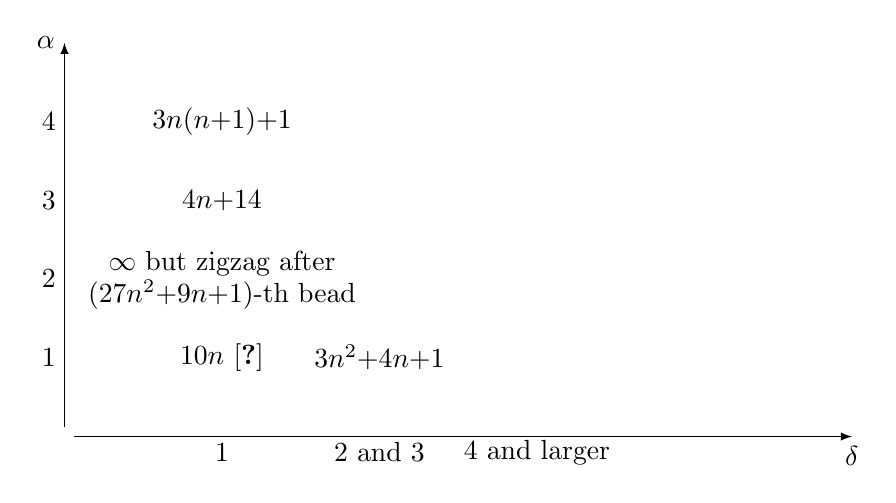
\begin{tikzpicture}

\node (origin) at (0, 0) {};

\draw[-latex] (origin) -- ++(0:10) node[below] {$\delta$}; 
\node at (2, -0.2) {1};
\node at (4, -0.2) {2 and 3};
\node at (6, -0.2) {4 and larger}; 
\draw[-latex] (origin) -- ++(90:5) node[left] {$\alpha$}; 
\node at (-0.2, 1) {1};
\node at (-0.2, 2) {2};
\node at (-0.2, 3) {3};
\node at (-0.2, 4) {4};

%Results
\node at (2, 4) {$3n(n{+}1){+}1$};
\node at (2, 3) {$4n{+}14$};
\node at (2, 2.2) {$\infty$ but zigzag after};
\node at (2, 1.8) {$(27n^2{+}9n{+}1)$-th bead};
\node at (2, 1) {$10n$ \cite{DHOPRSST2018}};

\node at (4, 1) {$3n^2{+}4n{+}1$};

\end{tikzpicture}
\caption{Upper bounds on the length of a conformation foldable by a deterministic unary oritatami system at delay $\delta$ and arity $\alpha$.
At any combination of delay and arity without anything written, no upper bound is known yet.
}
\label{fig:summary}
\end{figure}
In this paper, we will solve this problem  completely at delay 1 and partially at arity 1 in Sect.~\ref{sect:upper}. 
At delay 1, we will provide a quadratic upper bound $3n(n+1)+1$ for the case of arity being 4, while a linear upper bound $4n+14$ for arity 3. 
At the delay 1 and arity 2, one infinite structure turns out to be foldable deterministically, which is the zigzag conformation shown in Fig.~\ref{TTT_zigzag}. 
At arity 1, we will prove that at delay 2 or 3, the upper bound is $(3n+1)(n+1)$. 
Upper bounds for longer delays remain open. These results as well as known upper bounds are summarized in Fig.~\ref{fig:summary}. 
As shown at the end of Sect.~\ref{sec:preliminaries}, the stabilization of the first $t$ beads of transcript by a deterministic oritatami system can be simulated by a deterministic Turing machine within $t^3$ steps (Corollary~\ref{cor:DTIME3}). 
Thus, the above mentioned upper bounds show that at delay 1 and arity 1, 3, or 4, or at delay 2 or 3 and arity 1, the class of deterministic unary oritatami systems is not Turing universal. 
The Turing universal oritatami system by Geary et al. \cite{GeMeScSe2018} employs more than 500 types of beads. 
Thus, this weakness result is not surprising at all. 
The unary oritatami system might not be practical very much, though one bead may abstract an oligonucleotide (a short sequence of nucleotides), and in that case, unary transcript can be a repetitive but nonunary sequence, which is not so unrealistic in experiments (see \cite{GearyAndersen2014}). 
Nevertheless, this paper makes a first considerable step towards the characterization of non-Turing-universal oritatami systems. 

As a result of independent significance, we show that increasing the delay from 1 to 2 enables an oritatami system to yield a conformation of quadratic length in $n$ as long as 5 types of beads are available. 

%------------------------------------------------------
	\section{Preliminaries}\label{sec:preliminaries}
%------------------------------------------------------

Let $\Sigma$ be a finite set of types of abstract molecules, or \textit{beads}. 
A bead of type $a \in \Sigma$ is called an $a$-bead. 
By $\Sigma^*$ and $\Sigma^\omega$, we denote the set of finite sequences of beads and that of one-way infinite sequences of beads, respectively. 
The empty sequence is denoted by $\lambda$. 
Let $w = b_1 b_2 \cdots b_n \in \Sigma^*$ be a sequence of length $n$ for some integer $n$ and bead types $b_1, \ldots, b_n \in \Sigma$. 
The \textit{length} of $w$ is denoted by $|w|$, that is, $|w| = n$. 
For two indices $i, j$ with $1 \le i \le j \le n$, we let $w[i..j]$ refer to the subsequence $b_i b_{i+1} \cdots b_{j-1}b_j$; if $i = j$, then $w[i..i]$ is simplified as $w[i]$. 
For $k \ge 1$, $w[1..k]$ is called a \textit{prefix} of $w$. 

Oritatami systems fold their transcript, which is a sequence of beads, over the triangular grid graph $\mathbb{T} = (V, E)$ cotranscriptionally. 
We designate one point in $V$ as the origin $O$ of $\mathbb{T}$. 
For a point $p \in V$, let $\hexagon_p^d$ denote the set of points which lie in the regular hexagon of radius $d$ centered at the point $p$. 
Note that $\hexagon_p^d$ consists of $3d(d+1)+1$ points. 
A directed path $P = p_1 p_2 \cdots p_n$ in $\mathbb{T}$ is a sequence of \textit{pairwise-distinct} points $p_1, p_2, \ldots, p_n \in V$ such that $\{p_i, p_{i+1}\} \in E$ for all $1 \le i < n$. 
Its $i$-th point is referred to as $P[i]$. 
Now we are ready to abstract RNA single-stranded structures in the name of conformation. 
A \textit{conformation} $C$ (over $\Sigma$) is a triple $(P, w, H)$ of a directed path $P$ in $\mathbb{T}$, $w \in \Sigma^*$ of the same length as $P$, and a set of h-interactions $H \subseteq \bigl\{\{i, j\} \bigm| 1 \le i, i+2 \le j, \{P[i], P[j]\} \in E \bigr\}$. 
This is to be interpreted as the sequence $w$ being folded along the path $P$ in such a manner that its $i$-th bead $w[i]$ is placed at the $i$-th point $P[i]$ and the $i$-th and $j$-th beads are bound (by a hydrogen-bond-based interaction) if and only if $\{i, j\} \in H$. 
The condition $i+2 \le j$ represents the topological restriction that two consecutive beads along the path cannot be bound. 
The \textit{length} of $C$ is defined to be the length of its transcript $w$ (that is, equal to the length of the path $P$). 
A \textit{rule set} $R \subseteq \Sigma \times \Sigma$ is a symmetric relation over $\Sigma$, that is, for all bead types $a, b \in \Sigma$, $(a, b) \in R$ implies $(b, a) \in R$. 
A bond $\{i, j\} \in H$ is \textit{valid with respect to $R$}, or simply $R$-valid, if $(w[i], w[j]) \in R$. 
This conformation $C$ is \textit{$R$-valid} if all of its bonds are $R$-valid. 
For an integer $\alpha \ge 1$, $C$ is \textit{of arity $\alpha$} if it contains a bead that forms $\alpha$ bonds but none of its beads forms more. 
By $\mathcal{C}_{\le \alpha}(\Sigma)$, we denote the set of all conformations over $\Sigma$ whose arity is at most $\alpha$; its argument $\Sigma$ is omitted whenever $\Sigma$ is clear from the context. 

The oritatami system grows conformations by an operation called elongation. 
Given a rule set $R$ and an $R$-valid conformation $C_1 = (P, w, H)$, we say that another conformation $C_2$ is an elongation of $C_1$ by a bead $b \in \Sigma$, written as $C_1 \xrightarrow{R}_b C_2$, if $C_2 = (P p, wb, H \cup H')$ for some point $p \in V$ not along the path $P$ and set $H' \subseteq \bigl\{ \{i, |w|+1\} \bigm| 1 \le i < |w|, \{P[i], p\} \in E, (w[i], b) \in R \bigr\}$ of bonds formed by the $b$-bead; this set $H'$ can be empty. 
Note that $C_2$ is also $R$-valid. 
This operation is recursively extended to the elongation by a finite sequence of beads as: for any conformation $C$, $C \xrightarrow{R}_\lambda^* C$; and for a finite sequence of beads $w \in \Sigma^*$ and a bead $b \in \Sigma$, a conformation $C_1$ is elongated to a conformation $C_2$ by $wb$, written as $C_1 \xrightarrow{R}_{wb}^* C_2$, if there is a conformation $C'$ that satisfies $C_1 \xrightarrow{R}_w^* C'$ and $C' \xrightarrow{R}_b C_2$. 

An \textit{oritatami system} (OS) $\Xi = (\Sigma, R, \delta, \alpha, \sigma, w)$ is composed of
\begin{itemize}
\item a set $\Sigma$ of bead types, 
\item a rule set $R \subseteq \Sigma \times \Sigma$, 
\item a positive integer $\delta$ called the \textit{delay}, 
\item a positive integer $\alpha$ called the \textit{arity}, 
\item an initial $R$-valid conformation $\sigma \in C_{\le \alpha}(\Sigma)$ called the \textit{seed}, whose first bead is assumed to be at the origin $O$ without loss of generality, 
\item a (possibly infinite) \textit{transcript} $w \in \Sigma^* \cup \Sigma^\omega$, which is to be folded upon the seed by stabilizing beads of $w$ one at a time so as to minimize energy collaboratively with the succeeding $\delta{-}1$ nascent beads. 
\end{itemize}
The energy of a conformation $C = (P, w, H)$, denoted by $\Delta G(C)$, is defined to be ${-}|H|$; the more bonds a conformation has, the more stable it gets. 
The set $\mathcal{F}(\Xi)$ of conformations \textit{foldable} by the system $\Xi$ is recursively defined as: the seed $\sigma$ is in $\mathcal{F}(\Xi)$; and provided that an elongation $C_i$ of $\sigma$ by the prefix $w[1..i]$ be foldable (i.e., $C_0 = \sigma$), its further elongation $C_{i+1}$ by the next bead $w[i+1]$ is foldable if 
\begin{equation}\label{eq:OS_CF}
C_{i+1} \in \argmin_{
\substack{
C \in \mathcal{C}_{\le \alpha} s.t. \\
C_i \xrightarrow{R}_{w[i+1]}C \\
}
}
\min \Bigl\{ \Delta G(C') \Bigm|
C \xrightarrow{R}^*_{w[i+2...i+k]}C', k\le \delta, C' \in \mathcal{C}_{\le \alpha}
\Bigr\}.
\end{equation}
%
Then we say that the bead $w[i+1]$ and the bonds it forms are \textit{stabilized} according to $C_{i+1}$. 
Note that an arity-$\alpha$ oritatami system cannot fold any conformation of arity larger than $\alpha$. 
A conformation foldable by $\Xi$ is \textit{terminal} if none of its elongations is foldable by $\Xi$. 
The oritatami system $\Xi$ is \textit{deterministic} if for all $i \ge 0$, there exists at most one $C_{i+1}$ that satisfies \eqref{eq:OS_CF}. 
A deterministic oritatami system folds into a unique terminal conformation. 
An oritatami system with the empty rule set just folds into an arbitrary elongation of its seed nondeterministically. 
Thus, the rule set is reasonably assumed non-empty. 

In this paper, we considerably focus on the unary oritatami system. 
An oritatami system is \textit{unary} if it involves only one type of bead, say $a$, that is, $\Sigma = \{a\}$. 
Its rule set is $R = \{(a, a)\}$. 
Its transcript is a sequence of $a$-beads so that nothing can be hardcoded on it. 


\begin{proposition}\label{prop:check_validity}
	For any rule set $R$, arity $\alpha$ and conformation $C = (P,w,H)$ it is possible to check whether $C$ is $R$-valid and whether $C\in \mathcal{C}_{\leq \alpha}$ in time $\mathcal{O}(|H|\cdot|w|\cdot|R|)$.
\end{proposition}
\begin{proof}
	To check whether $C$ is $R$-valid:
	\begin{enumerate}
		\item FOR each $(i,j)\in H$:
		\item \hspace{1cm} IF $(w[i],w[j])\notin R$ THEN answer NO and HALT
		\item answer YES and HALT
	\end{enumerate}	
	Checking the condition in 2. can be done in $\mathcal{O}(|w|\cdot|R|)$ time for any reasonable representation of $w$ and $R$, hence the whole process takes $\mathcal{O}(|H|\cdot |w|\cdot|R|)$ time.	
	To check the arity constraint $C\in \mathcal{C}_{\leq \alpha}$: 
	\begin{enumerate}
		\item FOR each $i\in \{1,\dots,|w|\}$:
		\item \hspace{1cm} IF $\mathrm{degree}(i)=|\{j | (i,j)\in H \}|>\alpha$ THEN answer NO and HALT
		\item answer YES and HALT
	\end{enumerate}	
	Checking the condition in 2. can be done in $\mathcal{O}(|H|)$ time for any reasonable representation of $H$, hence the whole process takes $\mathcal{O}(|w|\cdot|H|)$ time.
	\qed
\end{proof}

\begin{theorem}\label{thm:OS_to_2dTM}
	There is an algorithm that simulates any deterministic oritatami system $\Xi = (\Sigma, R, \delta, \alpha, \sigma, w)$ in time $2^{\mathcal{O}(\delta)}\cdot |R|\cdot|w|$. 
\end{theorem}
\begin{proof}
	Take any step in the computation, up to which some $i \ge 0$ first beads of $w$ have been stabilized, with the last bead at a point $p$. 
	The number of all possible elongations of the current conformation by the next $\delta$-beads is $(6 \times 5^{\delta-1}) \times ((2^4)^{\delta-1} \times 2^5) \in 2^{O(\delta)}$. 
	By Proposition~\ref{prop:check_validity}, we can check for each of these elongations whether its arity is at most $\alpha$ or not and whether it is $R$-valid or not in time $\mathcal{O}((2^4)^{\delta-1}\cdot2^5\cdot \delta\cdot|R|)=2^{\mathcal{O}(\delta)}\cdot|R|$.  Therefore, the total running time is $2^{\mathcal{O}(\delta)}\cdot |R|\cdot|w|$.
	\qed
\end{proof}

\begin{corollary}\label{cor:DTIME3}
	For fixed $\delta$, the class of problems solvable by deterministic oritatami systems $(\Sigma, R, \delta, \alpha, \sigma, w)$ is included in $\mathrm{DTIME}(|w|^3)$.
\end{corollary}
\begin{proof}
	The claim follows from Theorem~\ref{thm:OS_to_2dTM} and the fact that $|R|$ is implicitly bounded by $|w|^2$.
	\qed
\end{proof}

%\begin{corollary}\label{polytranscript}
%	Let $k$ be a non-negative number. Let $\Sigma$, $H$, $\delta$, $\alpha$ be fixed and the transcript length bounded polynomially by the seed length, i.e., $|w|\in O(|\sigma|^k)$. Then, the language of seeds $\sigma$ accepted by an OS $(\Sigma, R, \delta, \alpha, \sigma, w)$ is in $\mathrm{DTIME}(|\sigma|^{2k})$.
%\end{corollary}

%If the transcript length is polynomially bounded by the seed length, than the accepted language is in $\mathrm{P}$. 

Considering the following decision problem: given an oritatami system, integer $i$, and a point $p$, decides whether the bead $w[i]$ is stabilized at $p$. 
By Corollary~\ref{cor:DTIME3}, this problem is in $\mathrm{P}$ for a fixed delay $\delta$.
Because of the time hierarchy theorems, we know that $\mathrm{P}\subsetneq \mathrm{EXP}$ (see, e.g., \cite{AroraBarak2009}), so we can conclude that OS which cannot deterministically fold transcripts of length exponential in the length of the seed are not computationally universal.


\section{Quadratic lower bound for delay 2, arity 1}\label{sect:lower}



%\subsection{$\alpha = 1$, arbitrary alphabets}
First we present a lower bound construction for arity $1$ systems. At $\alpha=1$, having delay $\delta=2$ allows the deterministic folding of quadratic length transcripts compared with $\delta=1$, where, as stated before, the maximum length is linear in the length of the seed. We demonstrate this with an infinite family of OS, which fold deterministically a transcript of length $\frac{(n-1)^2}{4}$ starting from a given seed of length $n$.

Consider the following $\delta=2$, $\alpha=1$ system with bead types $\{0,1,2,3,4\}$ and attraction rules $\{(1,1),(2,2), (3,3),(4,4)\}$. Let the seed $\sigma$ be a conformation of a $4k+1$ long bead sequence of the form $(1020)^k0$, such that bead $\sigma[i]$ of the seed is stabilized at point $(i,0)$, for all $1\leq i\leq 4k-1$. Bead $4k$ is at $(4k-1,-1)$ and bead $4k+1$ is at $(4k,0)$.
\vspace{0.1cm}

The transcript is $w=\mathrm{row}_1\cdots \mathrm{row}_{2k}$, where $\mathrm{row}_\ell$, for $\ell\in \{1,\dots, 2k\}$ is given in the table of Fig.~\ref{table:transcript}.
\begin{figure}[h]
	\begin{minipage}{.49\textwidth}
		%\centering
		\begin{tabular}{l|l}
			\multicolumn{2}{c}{Transcript $w$}\\
			\multicolumn{2}{c}{}  \\
			$k$ odd & \hspace{0.3cm} $k$ even\\\hline
			& \\
			$(2413)^{k-1}241$\hspace{0.3cm} & \hspace{0.3cm} $(2413)^{k-1}241$\\
			$(4231)^{k-1}4$   &  \hspace{0.3cm} $(4231)^{k-1}4$  \\
			$(1324)^{k-2}132$ &  \hspace{0.3cm} $(1324)^{k-2}132$\\
			$(3142)^{k-2}3$   &  \hspace{0.3cm} $(3142)^{k-2}3$ \\
			\vdots			 &  \hspace{0.3cm} \vdots\\
			$(1324)^1 132$	 &  \hspace{0.3cm} $(2413)^{1} 241$\\
			$(3142)^1 3$		 & \hspace{0.3cm} $(4231)^1 4$\\
			$(2413)^0 241$	 &  \hspace{0.3cm} $(1324)^0 132$\\
			$(4231)^0 4$		 & \hspace{0.3cm} $(3142)^0 3$\\
		\end{tabular}
	\end{minipage}
	%\scriptsize
	\begin{minipage}{.49\textwidth}
		%\centering
		\begin{tabular}{|l|c|}
			\hline
			\hspace{1.2cm}row $\ell$ & $\ell\mod 4$ \\\hline
			 & \\
			\hspace{0.1cm}$(2413)^{k-\lfloor (\ell+1)/2\rfloor}241$ \hspace{0.1cm} &  $\textrm{ }\ell\equiv 1\mod 4\textrm{ }$\\
			\hspace{0.1cm}$(4231)^{k-\lfloor (\ell+1)/2\rfloor}4$   &  $\textrm{ }\ell\equiv 2 \mod 4\textrm{ }$ \\
			\hspace{0.1cm}$(1324)^{k-\lfloor (\ell+1)/2\rfloor}132$ &  $\textrm{ }\ell\equiv 3 \mod 4\textrm{ }$ \\
			\hspace{0.1cm}$(3142)^{k-\lfloor (\ell+1)/2\rfloor}3$   &  $\textrm{ }\ell\equiv 4 \mod 4\textrm{ }$ \\\hline
		\end{tabular}
	
	\end{minipage}
	\caption{Transcript of pyramid-like conformation at delay $2$, arity $1$.}
	\label{table:transcript}
\end{figure}

The transcript above is written in rows which correspond to beads in the conformation stabilized along the same row on the grid. To simplify the argument we will use \textit{row} both for the transcript above and for the conformation it stabilizes in (note that in the figure the row index grows from bottom to top). 

Row $1$ is of length $4k-1$ and row $\ell+1$ is two beads shorter than row $\ell$, so the length of the whole transcript is $|w|=4k^2=\frac{(4k+1-1)^2}{4}=\frac{(|\sigma|-1)^2}{4}$. As an example, see Fig.~\ref{CI:big}, where $k=5$, so the length of the seed is $4k+1=21$ and the transcript is $4k^2 = 100$ beads long.

\begin{figure}
	\centering
	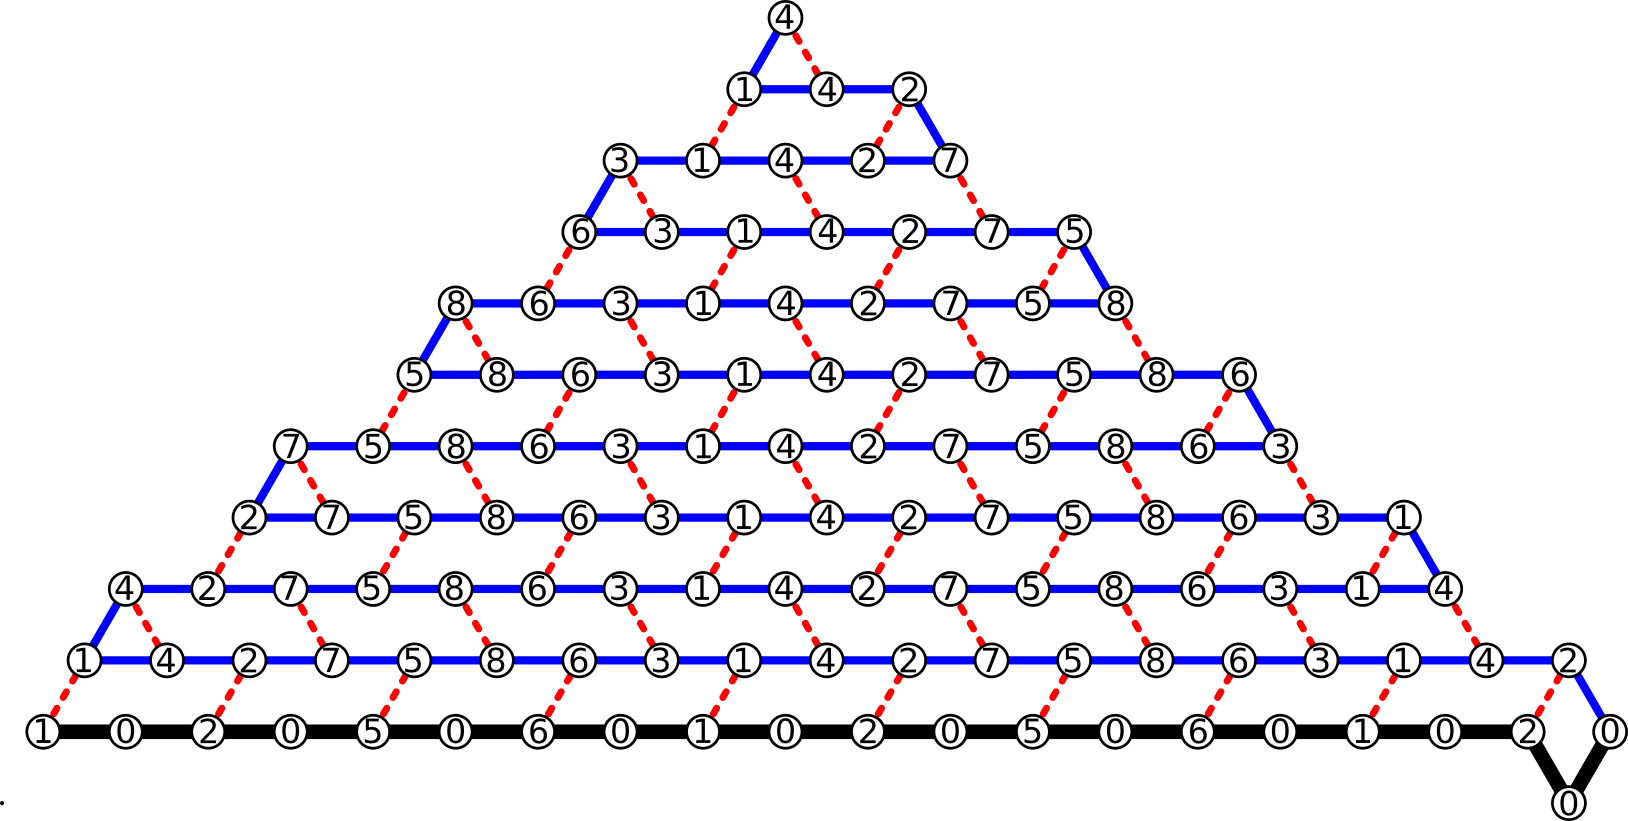
\includegraphics[width=0.7\linewidth]{./Fig/CI_NumbersNew}
	\caption{Quadratic length transcript folding deterministically into pyramid shape. Seed: thick black path. Transcript: thin blue path. Bonds: dashed red lines. }
	\label{CI:big}
\end{figure}


Stabilizing the first bead of row $j$ goes as follows (see Fig.~\ref{CI:turn}):
%\begin{itemize}
%	\item $\bf j\equiv 1\mod 4$: the first two beads are $24$, and the preceding bead is stabilized at $(4k-\frac{j-1}{2}, j-1)$. The $2$ can only bind to the $2$ which occurred two beads before at $(4k-\frac{j+1}{2}, j-1)$, and $4$ cannot bind anywhere, so the $2$ is stabilized at $(4k-\frac{j-1}{2},j)$.
%\end{itemize}

\begin{center}
	\begin{tabular}{|c|c|c|c|c|@{}m{0pt}@{}}
		%\renewcommand{\arraystretch}{2}
	$j\mod 4$					& first bead 	& predecessor at		& first bead binds to		& first stabilizes at\\
						\hline
	$\equiv 1$	& 2		& $(4k-\frac{j-1}{2}, j-1)$		& $(4k-\frac{j+1}{2}, j-1)$	& $(4k-\frac{j+1}{2}, j)$& $\mathrm{ }$\newline $\mathrm{ }$\\
	\hline
	$\equiv 2$	& 4				& $(\frac{3j}{2}-1,j-1)$		& $(\frac{3j}{2},j-1)$		& $(\frac{3j}{2},j)$ & $\mathrm{ }$\newline $\mathrm{ }$\\
	\hline
	$\equiv 3$	& 1				& $(4k-\frac{j-1}{2}, j-1)$		& $(4k-\frac{j+1}{2}, j-1)$	& $(4k-\frac{j+1}{2}, j)$ & $\mathrm{ }$\newline $\mathrm{ }$ \\
	\hline
	$\equiv 4$	& 3				& $(\frac{3j}{2}-1,j-1)$		& $(\frac{3j}{2},j-1)$		& $(\frac{3j}{2},j)$ & $\mathrm{ }$\newline $\mathrm{ }$ \\
	\hline		
	\end{tabular}
\end{center}



%The first bead of the transcript is type $2$ and it has to be fixed next to $(4k,0)$. The second bead is type $4$, which cannot form a bond with anything in the conformation so far. The only possibility of forming a bond is if the $2$-bead is placed at $(4k,1)$ and it bonds with the $2$-bead of the seed at $(4k-1,0)$. The next to be stabilized is a $4$-bead, and since it cannot form any bond, the conformation with the highest number of bonds is when the one after, a $1$-bead, is at $(4k-2,1)$ bonding with $(4k-3,0)$, which stabilizes the preceding $4$-bead at $(4k-1,1)$ (see Fig.~\ref{CI:1-4}, (a)-(b)).



\begin{figure}
	\begin{minipage}{.35\textwidth}
		\centering
		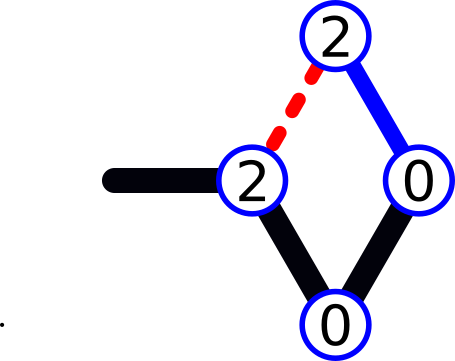
\includegraphics[align=c,height=1in]{./Fig/CI_1n}\\
		\bigskip
		
		(a) First transcript bead
	\end{minipage}%
	\begin{minipage}{.2\textwidth}
		\centering
		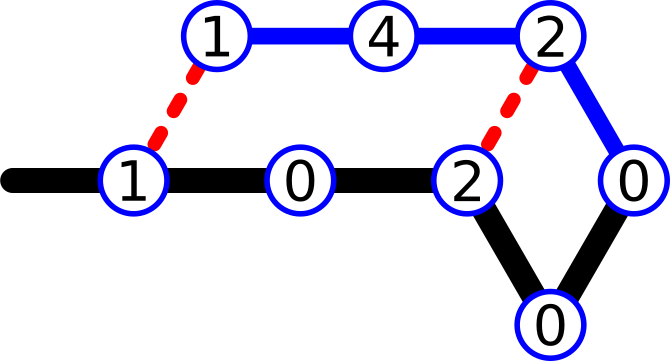
\includegraphics[align=c,height=0.7in]{./Fig/CI_2n}\\
		\bigskip
		
		(b) Second bead
	\end{minipage}
	\begin{minipage}{.4\textwidth}
		\centering
		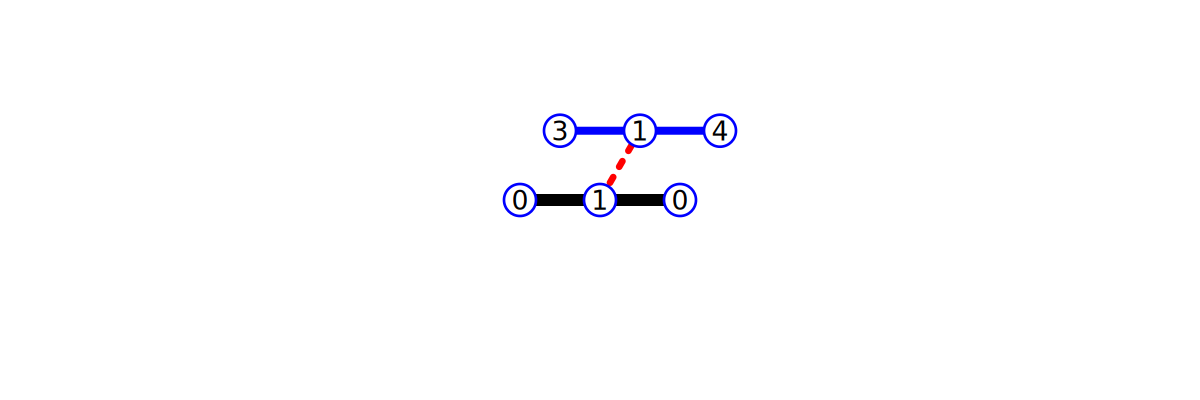
\includegraphics[align=c,height=0.5in]{./Fig/CI_3n}
		\bigskip
		\vspace{0.1in}
		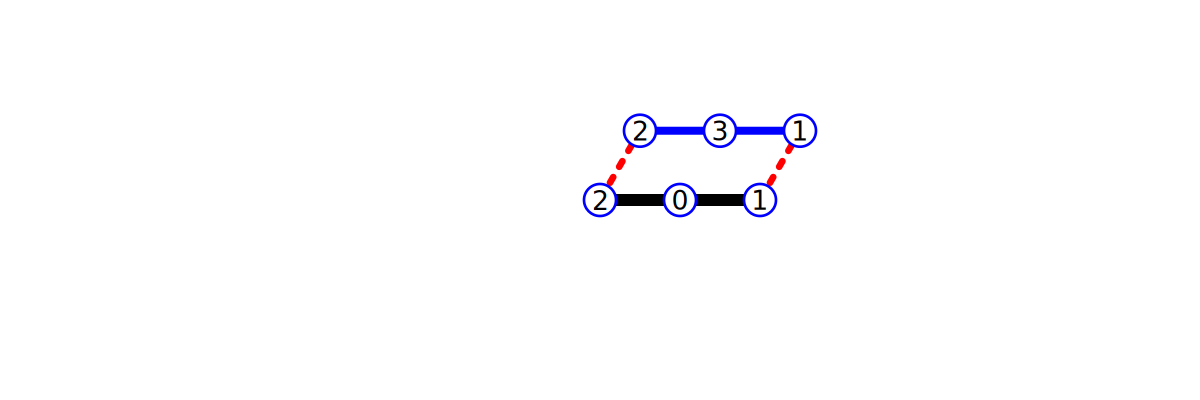
\includegraphics[align=c,height=0.5in]{./Fig/CI_4n}
		\bigskip
		
		(c) Portions of row $1$
	\end{minipage}
	\caption{Fixing transcript beads in odd rows}
	\label{CI:1-4}
\end{figure}


As for the other beads, in rows $j\equiv 1,3\mod 4$, beads of type $1$ and $3$ bind to a bead in row $j-1$. In rows $j\equiv 2,4\mod 4$ beads of type $2$ and $4$ can bind to a bead in row $j-1$.  This is true for row $1$, because beads of type $1$ and $3$ from row $1$ can only bind to every second bead of the seed, whereas beads of type $2$ and $4$ from row $1$ cannot bind to anything (Fig.~\ref{CI:1-4}, (c)). Once this dynamic holds for a row, it holds inductively for the next, as a bead that binds to another loses its only free hand at arity $1$.

Within one row of the transcript, no bead can bind to a preceding bead, because if there is a previous bead of the same type in that row, it is stabilized at a distance of four and the system has delay $2$.

By the arguments above, the beads in row $i$ of the transcript are stabilized along row $i$ on the grid, forming the pyramid-like conformation from Fig.~\ref{CI:big}.


\begin{figure}
	\centering
	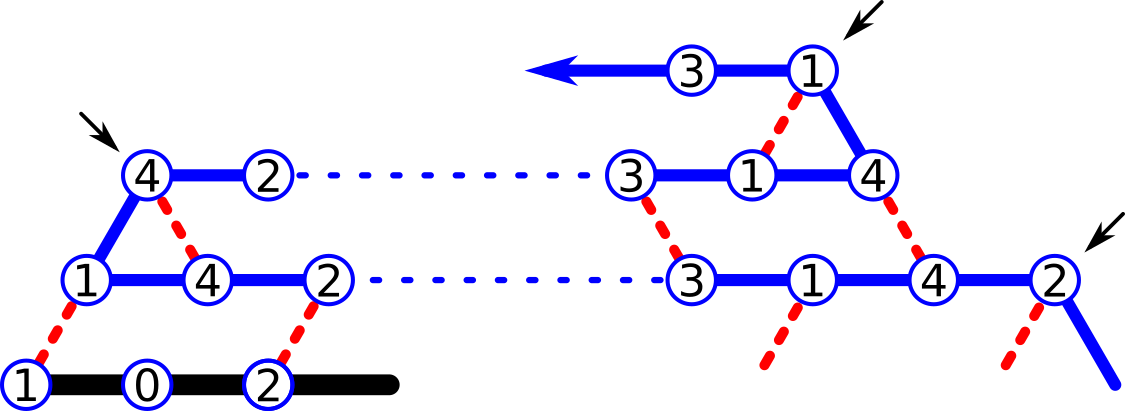
\includegraphics[width=0.7\linewidth]{./Fig/CI_turnn}
	\caption{Beads $4k, 8k-2, \dots$ stabilize at turning points because the bead two positions before is the same type and has a free hand.}
	\label{CI:turn}
\end{figure}





%\section{Case of arity $1$}\label{sect:arity1}


%

\subsection{$\alpha = 1$, arbitrary alphabets}
First we present a lower bound construction for arity $\alpha=1$ systems. At $\alpha=1$, allowing delay $\delta=2$ increases the power of OS compared with $\delta=1$, if at least four bead types are allowed. We demonstrate this with an infinite family of OS, which fold deterministically a transcript of length $\frac{(n-1)^2}{4}$ starting from a given seed of length $n$.

Consider the following $\delta=2$, $\alpha=1$ system with bead types $\{0,1,2,3,4\}$ and attraction rules $\{(1,1),(2,2), (3,3),(4,4)\}$. Let the seed $\sigma$ be a conformation of a $4k+1$ long bead sequence of the form $(1020)^k0$, such that bead $\sigma[i]$ of the seed is stabilized at point $(i,0)$, for all $1\leq i\leq 4k-1$. Bead $4k$ is at $(4k-1,-1)$ and bead $4k+1$ is at $(4k,0)$.

\noindent The transcript is
\begin{center}
	
	%\scriptsize
	\begin{tabular}{llll}
		& $k$ odd &  & $k$ even\\
		$w=$\hspace{1cm} & $(2413)^{k-1}241$ & \hspace{1cm} &  $(2413)^{k-1}241$\\
		     & $(4231)^{k-1}4$   & &  $(4231)^{k-1}4$  \\
		     & $(1324)^{k-2}132$ & &  $(1324)^{k-2}132$\\
		     & $(3142)^{k-2}3$   & &  $(3142)^{k-2}3$ \vspace{5pt}\\
		     
		     & $(2413)^{k-3}241$ & &  $(2413)^{k-3}241$\\
		     & $(4231)^{k-3}4$   & &  $(4231)^{k-3}4$  \\
		     & $(1324)^{k-4}132$ & &  $(1324)^{k-4}132$\\
		     & $(3142)^{k-4}3$   & &  $(3142)^{k-4}3$\\
			 & \vdots			 & &  \vdots\\
			 & $(2413)^{2} 241$	 & &  $(2413)^{1} 241$\\
			 & $(4231)^2 4$		 & &  $(4231)^1 4$\\
			 & $(1324)^1 132$	 & &  $(1324)^0 132$\\
			 & $(3142)^1 3$		 & &  $(3142)^0 3$\\
			 & $(2413)^0 241$	 & & \\
			 & $(4231)^0 4$  	 & 
	\end{tabular}
	
\end{center}
The transcript above is written in rows which correspond to beads in the conformation stabilized along the same row on the grid. To simplify the argument we will use \textit{row} both for the transcript above and for the conformation it stabilizes in. In line with this, row $\ell\in \{1,\dots, 2k\}$ is as follows:  
\begin{center}
	\begin{tabular}{llll}
							& row $\ell$ & 			& $\ell\mod 4$ \\
			& $(2413)^{k-\lfloor (\ell+1)/2\rfloor}241$ & \hspace{1cm} &  $\ell\equiv 1\mod 4$\\
							& $(4231)^{k-\lfloor (\ell+1)/2\rfloor}4$   & &  $\ell\equiv 2 \mod 4$ \\
							& $(1324)^{k-\lfloor (\ell+1)/2\rfloor}132$ & &  $\ell\equiv 3 \mod 4$\\
							& $(3142)^{k-\lfloor (\ell+1)/2\rfloor}3$   & &  $\ell\equiv 4 \mod 4$ 
	\end{tabular}
\end{center}
so $w=\mathrm{row}_1\cdots \mathrm{row}_{2k}$. Row $1$ is of length $4k-1$ and row $\ell+1$ is two beads shorter than row $\ell$, so the length of the whole transcript is $|w|=4k^2=\frac{(4k+1-1)^2}{4}=\frac{(|\sigma|-1)^2}{4}$. As an example, see Fig.~\ref{CI:big}, where $k=5$, so the length of the seed is $4k+1=21$ and the transcript is $4k^2 = 100$ beads long.

\begin{figure}
	\centering
	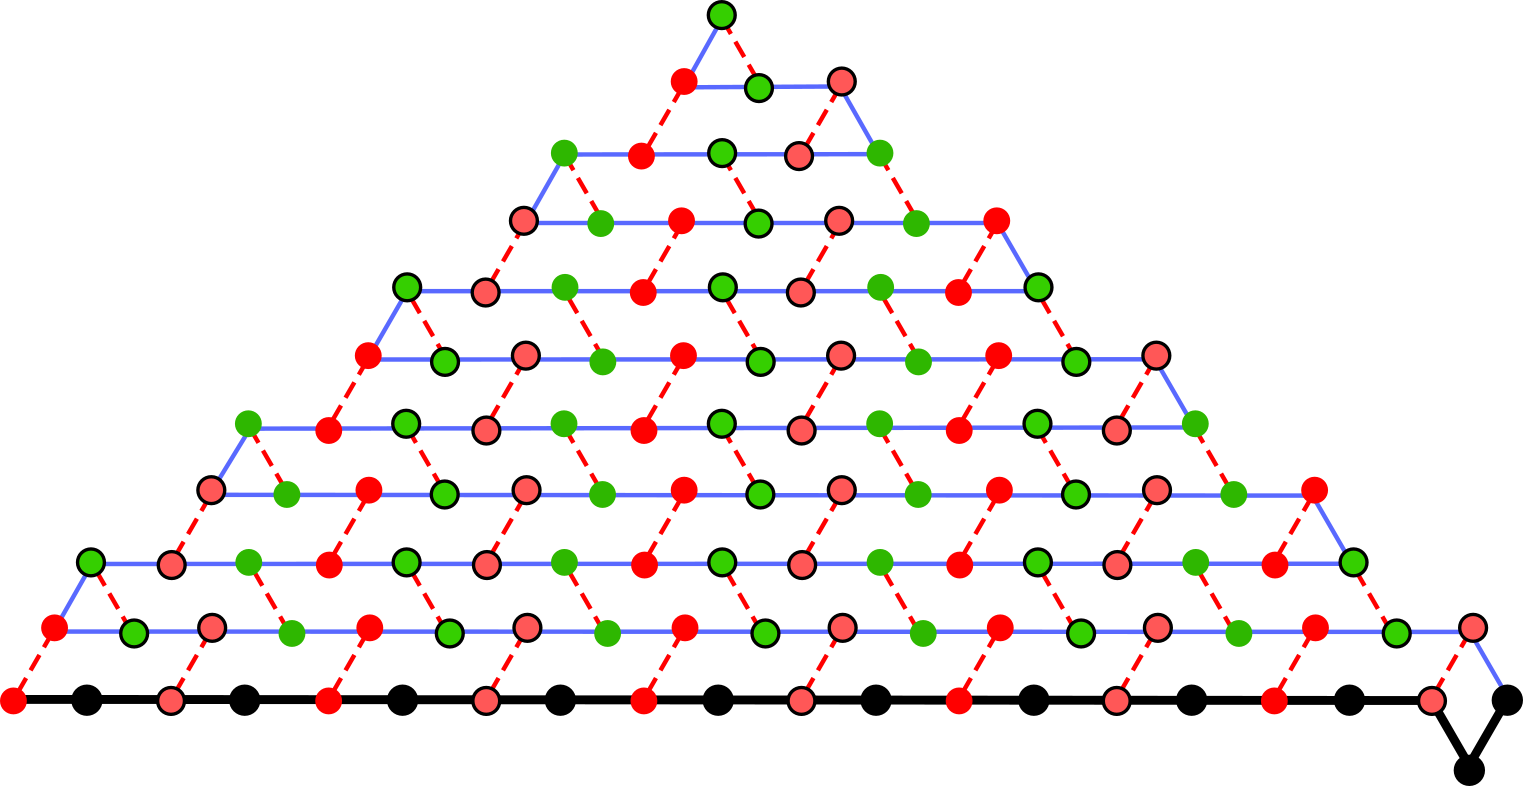
\includegraphics[width=0.9\linewidth]{./Fig/chichenBig}
	\caption{Quadratic length transcript folding deterministically into pyramid shape. Seed: thick black path. Transcript: thin blue path. Bonds: dashed red lines. Beads: '$0$' black, '$1$' red, '$2$' red with black contour, '$3$' green, '$4$' green with black contour.}
	\label{CI:big}
\end{figure}


Stabilizing the first bead of row $j$ goes as follows (see Fig.~\ref{CI:turn}):
%\begin{itemize}
%	\item $\bf j\equiv 1\mod 4$: the first two beads are $24$, and the preceding bead is stabilized at $(4k-\frac{j-1}{2}, j-1)$. The $2$ can only bind to the $2$ which occurred two beads before at $(4k-\frac{j+1}{2}, j-1)$, and $4$ cannot bind anywhere, so the $2$ is stabilized at $(4k-\frac{j-1}{2},j)$.
%\end{itemize}

\begin{center}
	\begin{tabular}{|c|c|c|c|c|@{}m{0pt}@{}}
		%\renewcommand{\arraystretch}{2}
	$j\mod 4$					& first bead 	& predecessor at		& first bead binds to		& first stabilizes at\\
						\hline
	$\equiv 1$	& 2		& $(4k-\frac{j-1}{2}, j-1)$		& $(4k-\frac{j+1}{2}, j-1)$	& $(4k-\frac{j+1}{2}, j)$& $\mathrm{ }$\newline $\mathrm{ }$\\
	\hline
	$\equiv 2$	& 4				& $(\frac{3j}{2}-1,j-1)$		& $(\frac{3j}{2},j-1)$		& $(\frac{3j}{2},j)$ & $\mathrm{ }$\newline $\mathrm{ }$\\
	\hline
	$\equiv 3$	& 1				& $(4k-\frac{j-1}{2}, j-1)$		& $(4k-\frac{j+1}{2}, j-1)$	& $(4k-\frac{j+1}{2}, j)$ & $\mathrm{ }$\newline $\mathrm{ }$ \\
	\hline
	$\equiv 4$	& 3				& $(\frac{3j}{2}-1,j-1)$		& $(\frac{3j}{2},j-1)$		& $(\frac{3j}{2},j)$ & $\mathrm{ }$\newline $\mathrm{ }$ \\
	\hline		
	\end{tabular}
\end{center}



%The first bead of the transcript is type $2$ and it has to be fixed next to $(4k,0)$. The second bead is type $4$, which cannot form a bond with anything in the conformation so far. The only possibility of forming a bond is if the $2$-bead is placed at $(4k,1)$ and it bonds with the $2$-bead of the seed at $(4k-1,0)$. The next to be stabilized is a $4$-bead, and since it cannot form any bond, the conformation with the highest number of bonds is when the one after, a $1$-bead, is at $(4k-2,1)$ bonding with $(4k-3,0)$, which stabilizes the preceding $4$-bead at $(4k-1,1)$ (see Fig.~\ref{CI:1-4}, (a)-(b)).



\begin{figure}
	\begin{minipage}{.35\textwidth}
		\centering
		\includegraphics[align=c,height=1in]{./Fig/CI_1}\\
		\bigskip
		
		(a) First transcript bead
	\end{minipage}%
	\begin{minipage}{.2\textwidth}
		\centering
		\includegraphics[align=c,height=0.7in]{./Fig/CI_2}\\
		\bigskip
		
		(b) Second bead
	\end{minipage}
	\begin{minipage}{.4\textwidth}
		\centering
		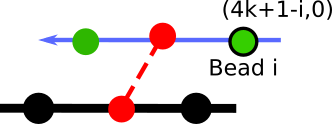
\includegraphics[align=c,height=0.5in]{./Fig/CI_3}
		\bigskip
		\vspace{0.1in}
		\includegraphics[align=c,height=0.5in]{./Fig/CI_4}
		\bigskip
		
		(c) Bead $i+1$, when bead $i$ is $B_{3,4}$ and $B_{1,2}$, respectively
	\end{minipage}
	\caption{Fixing transcript beads in odd rows}
	\label{CI:1-4}
\end{figure}


As for the other beads, in rows $j\equiv 1,3\mod 4$, beads of type $1$ and $3$ bind to a bead in row $j-1$. In rows $j\equiv 2,4\mod 4$ beads of type $2$ and $4$ can bind to a bead in row $j-1$.  This is true for row $1$, because beads of type $1$ and $3$ from row $1$ can only bind to every second bead of the seed, whereas beads of type $2$ and $4$ from row $1$ cannot bind to anything (Fig.~\ref{CI:1-4}, (c)). Once this dynamic holds for a row, it holds inductively for the next, as a bead that binds to another loses its only free hand at arity $1$.

Within one row of the transcript, no bead can bind to a preceding bead, because if there is a previous bead of the same type in that row, it is stabilized at a distance of four and the system has delay $2$.

By the arguments above, the beads in row $i$ of the transcript are stabilized along row $i$ on the grid, forming the pyramid-like conformation from Fig.~\ref{CI:big}.


\begin{figure}
	\centering
	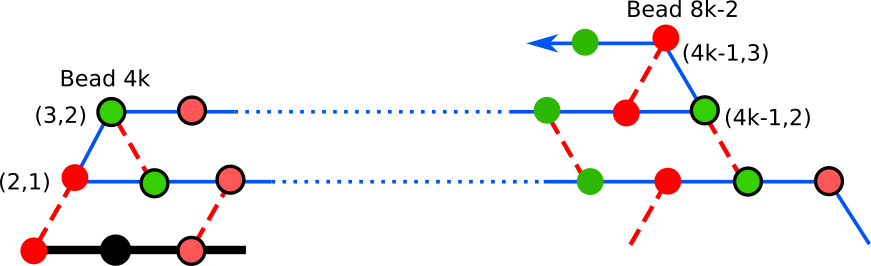
\includegraphics[width=0.7\linewidth]{./Fig/CI_turn}
	\caption{Beads $4k, 8k-2, \dots$ stabilize at turning points because the bead two positions before is the same type and has a free hand.}
	\label{CI:turn}
\end{figure}




\subsection{$\alpha = 1$, unary}

Let the point where the first transcript bead was fixed be $p$ and let $n=|\mathrm{seed}|+1$. We will argue about the situation when the first bead is stabilized outside $\hexagon_p^n$ (a hexagon of radius $n$). Let this be the $i$th bead of the transcript. Without loss of generality, we can translate the origin $(0,0)$ to the coordinates of bead $i-1$ (which is still in $\hexagon_p^n$), and we can assume that the bead outside the hexagon is fixed at $(1,1)$ (see Fig.~\ref{fig:hexagonOut}).
\begin{figure}
	\centering
	\includegraphics[width=0.3\linewidth]{./Fig/hexagonOut}
	\caption{$\hexagon_p^n$ and the position $(1,1)$ of the first bead fixed outside of it.}
	\label{fig:hexagonOut}
\end{figure}

In the elongation that places bead $i$ at $(1,1)$ there are two possibilities:
\begin{itemize}
	\item $i$ forms a bond with a bead at $(1,0)$.
	\item  $i$ does not bond to anything and $i+1$ is at $(2,1)$ bonding with a bead at $(2,0)$. If there is no bead at $(1,0)$, then placing $i$ at $(1,0)$ instead of $(1,1)$ results in the same number of bonds, leading to nondeterminism. Therefore, there has to be a bead at $(1,0)$ and it is inactive, otherwise it would bond to $i$. This is analogous to case 1. below.%as in Fig.~\ref{fig:hexagonOut1}.
	\begin{figure}
		\centering
		\includegraphics[width=0.2\linewidth]{./Fig/hexagonOut1}
		%\caption{}
		\label{fig:hexagonOut1}
	\end{figure}
	
\end{itemize}
 
%The only position with which $(1,1)$ can form a bond is $(1,0)$. This means that there is a bead at $(1,0)$, which bonds to bead $i$, otherwise there are other conformations in which beads $i$ and $i+1$ add one bond to the conformation, making the behavior nondeterministic.

The next bead, $i+1$, can be fixed at $(2,1)$ or at $(0,1)$ as all other possibilities result in nondeterministic behavior immediately, so we have two cases.

\begin{enumerate}
	\item bead $i+1$ is fixed at $(2,1)$ and can bond with a bead at $(2,0)$. Now consider bead $i+2$. For $i+1$ to be fixed at $(2,1)$, $i+2$ needs to form a bond somewhere, otherwise $i+2$ could go to $(2,1)$ forming the bond with the bead at $(2,0)$ and there would be two conformations with the maximal $1$ bond. The only possibility is that there is a bead at $(3,0)$ and $i+2$ can bond with it when placed at $(3,1)$. We can apply the same argument inductively: there is some $m\geq 0$ such that grid points $(\ell,0)$ are occupied by active beads, for all $\ell\in \{2,\dots,2+m\}$, and there is no bead at $(3+m,0)$. Such an $m$ exists, and it is not greater than $n$. Then, bead $i+\ell$ is fixed at $(\ell+1,1)$ and bonds with $(\ell+1,0)$. However, bead $i+2+m$ cannot be fixed anywhere, because $i+2+m$ and $i+3+m$ can only add one bond to the conformation, and that is possible either with $i+2+m \rightarrow (2+m,1)$, $i+3+m \rightarrow (3+m,1)$ or with $i+2+m \rightarrow (2+m,2)$, $i+3+m \rightarrow (2+m,1)$. 
	\begin{figure}
		\centering
		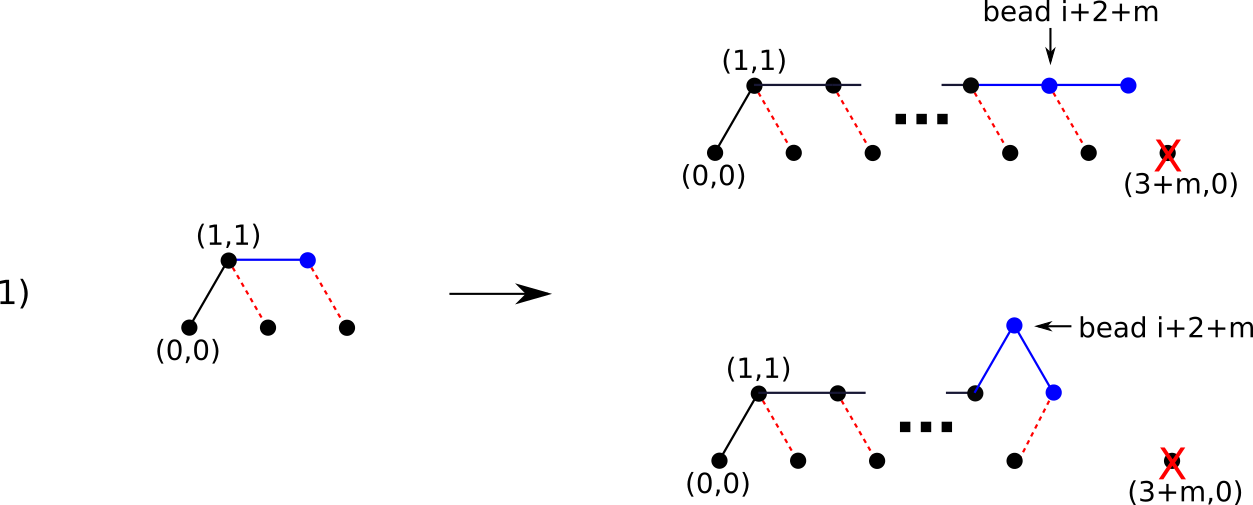
\includegraphics[width=0.6\linewidth]{./Fig/hexagonOut2}
		\caption{}
		\label{fig:hexagonout2}
	\end{figure}
	
	\item bead $i+1$ is fixed at $(0,1)$. This is only possible if
	\begin{enumerate}
		\item there is an inactive bead at $(-1,0)$ and an active one at $(-2,0)$. This case is symmetrical to (1).
		\item there is no bead at $(-1,0)$, bead $i+1$ can bond with bead $i-1$ at $(0,0)$ and the bead $i+2$ can be placed at $(-1,0)$ where it can bond with $(-2,0)$, $(-2,-1)$ or $(-1,-1)$. This leads to nondeterminism, because bead $i$ at $(-1,0)$ and bead $i+1$ at $(0,1)$ has two bonds, just as the original conformation.
		\item there is a bead at $(-1,0)$ and bead $i+1$ can bond with that or with bead $i-1$ at $(0,0)$. However, this means that placing bead $i$ at $(0,1)$ at bead $i+1$ at $(1,1)$ creates the same number of hydrogen bonds, thus resulting in bead $i$ not being placed deterministically.
		
	\end{enumerate}
\end{enumerate}




\begin{figure}
	\centering
	%\includegraphics[width=0.3\linewidth]{./hexagonOut1}
	%\hspace{10mm} %
	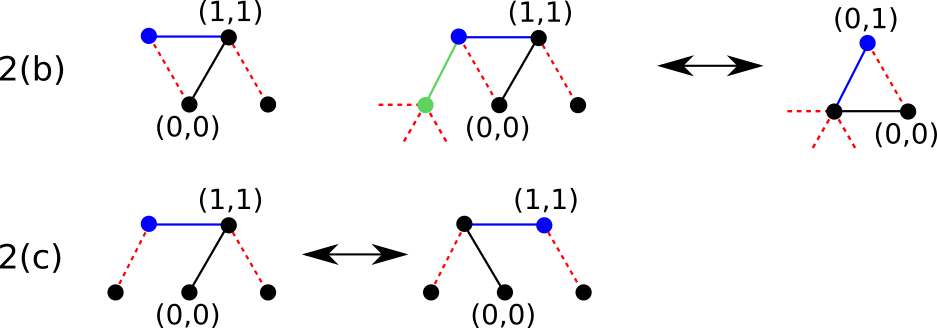
\includegraphics[width=0.6\linewidth]{./Fig/hexagonOut3}
	
	\caption{}
	\label{fig:hexagonOut2}
\end{figure}


\subsection{In the case of $\delta = 3$}

As before, the length of seed is $n$ and the seed will be inside $\hexagon_p^n$, the equilateral hexagon with a radius of $n$ and center $p$, the point where the first bead of the seed is fixed. We will begin our discussion by considering the moment when the first bead is fixed outside $\hexagon_p^n$. Let this bead be the $i$th one. 

\textbf{A.} First, let us assume that a fixed bead on a side of $\hexagon_p^n$ has a free hand, and bead $i$ binds to it. If the most stable conformation formed by beads $i, i+1, i+2$ has only two hydrogen bonds, it will be nondeterministic because there are at least two possibilities, see Fig.~\ref{fig:beadi}. Therefore, it needs to make three hydrogen bonds to deterministically stabilize $i$.\\

\begin{figure}
  \begin{center}
  \begin{tabular}{cc}
    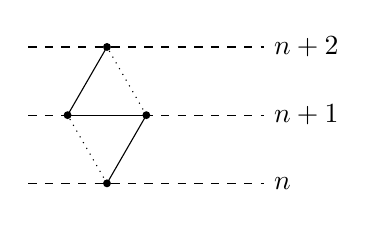
\begin{tikzpicture}
      \draw [dashed] (-1.0, 0.0) -- (2.0, 0.0);
      \fill (2.0, 0.0) node [right] {$n$};
      \draw [dashed] (-1.0, 0.866) -- (2.0, 0.866);
      \fill (2.0, 0.866) node [right] {$n+1$};
      \draw [dashed] (-1.0, 1.732) -- (2.0, 1.732);
      \fill (2.0, 1.732) node [right] {$n+2$};
      \fill (0,0) circle [radius = 0.05];
      \begin{scope}[shift = (0 : 0.0)]
        \foreach \theta in {60, 120}{
          \fill (0,0) [transform canvas = {shift = (\theta : 1.0)}] circle [radius = 0.05];
        }
        \draw (0 : 0.0) -- (60 : 1.0);
        \draw (60 : 1.0) -- (120 : 1.0);
        \draw [dotted] (0 : 0.0) -- (120 : 1.0);
      \end{scope}
      \begin{scope}[shift = (60 : 1.0)]
        \draw [dotted] (0 : 0.0) -- (120 : 1.0);
      \end{scope}
      \begin{scope}[shift = (120 : 1.0)]
        \foreach \theta in {60}{
        \fill (0,0) [transform canvas = {shift = (\theta : 1.0)}] circle [radius = 0.05];
        }
        \draw (0 : 0.0) -- (60 : 1.0);
      \end{scope}
    \end{tikzpicture}

    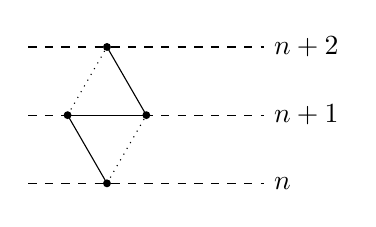
\begin{tikzpicture}
      \draw [dashed] (-1.0, 0.0) -- (2.0, 0.0);
      \fill (2.0, 0.0) node [right] {$n$};
      \draw [dashed] (-1.0, 0.866) -- (2.0, 0.866);
      \fill (2.0, 0.866) node [right] {$n+1$};
      \draw [dashed] (-1.0, 1.732) -- (2.0, 1.732);
      \fill (2.0, 1.732) node [right] {$n+2$};
      \fill (0,0) circle [radius = 0.05];
      \begin{scope}[shift = (0 : 0.0)]
        \foreach \theta in {60, 120}{
          \fill (0,0) [transform canvas = {shift = (\theta : 1.0)}] circle [radius = 0.05];
        }
        \draw [dotted] (0 : 0.0) -- (60 : 1.0);
        \draw (60 : 1.0) -- (120 : 1.0);
        \draw (0 : 0.0) -- (120 : 1.0);
      \end{scope}
      \begin{scope}[shift = (60 : 1.0)]
        \draw (0 : 0.0) -- (120 : 1.0);
      \end{scope}
      \begin{scope}[shift = (120 : 1.0)]
        \foreach \theta in {60}{
        \fill (0,0) [transform canvas = {shift = (\theta : 1.0)}] circle [radius = 0.05];
        }
        \draw [dotted](0 : 0.0) -- (60 : 1.0);
      \end{scope}
    \end{tikzpicture}
    \end{tabular}
    \caption{}
    \label{fig:beadi}
  \end{center}
\end{figure}

There are the two cases in which beads $i, i+1, i+2$ can have three bonds, see Fig.~\ref{fig:3bonds}. However, if it makes three bonds once, such as in Fig.~\ref{fig:3bonds}, it will need to make three bonds forever to be deterministic. Similarly to case 1. in the previous section, this becomes nondeterministic finally, as in Fig.~\ref{fig:hexcorner}, when it reaches a corner of $\hexagon_p^n$. Thus, the fixed bead on the side of an equilateral hexagon with a radius of $n$ has to make a hydrogen bond with a bead in an equilateral hexagon.

\begin{figure}
  \begin{center}
  \begin{tabular}{cc}
    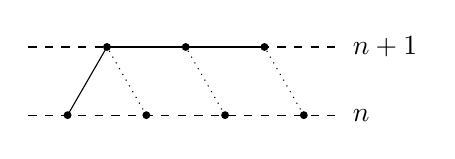
\begin{tikzpicture}
      \draw [dashed] (-0.5, 0.0) -- (3.5, 0.0);
      \fill (3.5, 0.0) node [right] {$n$};
      \draw [dashed] (-0.5, 0.866) -- (3.5, 0.866);
      \fill (3.5, 0.866) node [right] {$n+1$};
      \fill (0,0) circle [radius = 0.05];
      \begin{scope}[shift = (0 : 0.0)]
        \foreach \theta in {0, 60}{
          \fill (0,0) [transform canvas = {shift = (\theta : 1.0)}] circle [radius = 0.05];
        }
        \draw (0 : 0.0) -- (60 : 1.0);
      \end{scope}
      \begin{scope}[shift = (0 : 2.0)]
        \fill (0,0) circle [radius = 0.05];
        \foreach \theta in {0, 60, 120}{
          \fill (0,0) [transform canvas = {shift = (\theta : 1.0)}] circle [radius = 0.05];
        }
        \draw [dotted] (0 : 0.0) -- (120 : 1.0);
      \end{scope}
      \begin{scope}[shift = (60 : 1.0)]
          \draw (0 : 0.0) -- (0 : 2.0);
      \end{scope}
      \begin{scope}[shift = (0 : 1.0)]
          \draw [dotted] (0 : 0.0) -- (120 : 1.0);
      \end{scope}
      \begin{scope}[shift = (0 : 3.0)]
          \draw [dotted] (0 : 0.0) -- (120 : 1.0);
      \end{scope}
    \end{tikzpicture}

    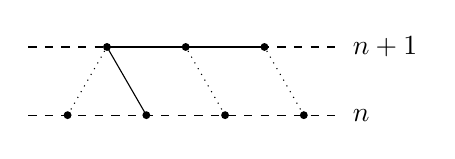
\begin{tikzpicture}
      \draw [dashed] (-1.5, 0.0) -- (2.5, 0.0);
      \fill (2.5, 0.0) node [right] {$n$};
      \draw [dashed] (-1.5, 0.866) -- (2.5, 0.866);
      \fill (2.5, 0.866) node [right] {$n+1$};
      \fill (0,0) circle [radius = 0.05];
      \begin{scope}[shift = (0 : 0.0)]
        \foreach \theta in {0, 60, 120, 180}{
          \fill (0,0) [transform canvas = {shift = (\theta : 1.0)}] circle [radius = 0.05];
        }
        \draw (0 : 0.0) -- (120 : 1.0);
      \end{scope}
      \begin{scope}[shift = (0 : 2.0)]
        \fill (0,0) circle [radius = 0.05];
        \foreach \theta in {120}{
          \fill (0,0) [transform canvas = {shift = (\theta : 1.0)}] circle [radius = 0.05];
        }
        \draw [dotted] (0 : 0.0) -- (120 : 1.0);
      \end{scope}
      \begin{scope}[shift = (120 : 1.0)]
          \draw (0 : 0.0) -- (0 : 2.0);
      \end{scope}
      \begin{scope}[shift = (0 : 1.0)]
          \draw [dotted] (0 : 0.0) -- (120 : 1.0);
      \end{scope}
      \begin{scope}[shift = (180 : 1.0)]
          \draw [dotted] (0 : 0.0) -- (60 : 1.0);
      \end{scope}
    \end{tikzpicture}
    \end{tabular}
    \caption{}
    \label{fig:3bonds}
  \end{center}
  	
\end{figure}

\begin{figure}
  \begin{center}
  \begin{tabular}{cc}
    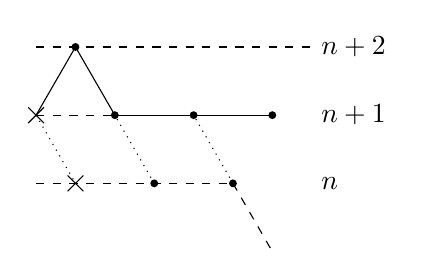
\begin{tikzpicture}
      \draw [dashed] (-0.5, 0.0) -- (2.0, 0.0);
      \fill (3.0, 0.0) node [right] {$n$};
      \draw [dashed] (-0.5, 0.866) -- (2.5, 0.866);
      \fill (3.0, 0.866) node [right] {$n+1$};
      \draw [dashed] (-0.5, 1.732) -- (3.0, 1.732);
      \fill (3.0, 1.732) node [right] {$n+2$};
      \fill (60 : 1.0) circle [radius = 0.05];
      \draw (-0.1,-0.1) -- (0.1,0.1);
      \draw (0.1,-0.1) -- (-0.1,0.1);
      \begin{scope}[shift = (120 : 1.0)]
        \draw (-0.1,-0.1) -- (0.1,0.1);
        \draw (0.1,-0.1) -- (-0.1,0.1);
      \end{scope}
      \begin{scope}[shift = (120 : 1.0)]
        \draw [dotted] (0 : 0.0) -- (300 : 1.0);
      \end{scope}
      \begin{scope}[shift = (60 : 1.0)]
        \draw (0.0, 0.0) -- (2.0, 0.0);
        \fill (2.0, 0.0) circle [radius = 0.05];
      \end{scope}
      \begin{scope}[shift = (0 : 2.0)]
        \draw [dashed] (0 : 0.0) -- (300 : 1.0);
      \end{scope}
      \begin{scope}[shift = (0 : 1.0)]
      \fill (0.0, 0.0) circle [radius = 0.05];
        \foreach \theta in {0, 60}{
          \fill (0,0) [transform canvas = {shift = (\theta : 1.0)}] circle [radius = 0.05];
        }
        \draw [dotted] (0 : 0.0) -- (120 : 1.0);
      \end{scope}
      \begin{scope}[shift = (0 : 2.0)]
        \draw [dotted] (0 : 0.0) -- (120 : 1.0);
      \end{scope}
      \begin{scope}[shift = (60 : 1.0)]
        \begin{scope}[shift = (120 : 1.0)]
          \fill (0.0, 0.0) circle [radius = 0.05];
          \draw (0 : 0.0) -- (240 : 1.0);
          \draw (0 : 0.0) -- (300 : 1.0);
        \end{scope}
      \end{scope}
    \end{tikzpicture}

    \begin{tikzpicture}
      \draw [dashed] (-0.5, 0.0) -- (2.0, 0.0);
      \fill (3.0, 0.0) node [right] {$n$};
      \draw [dashed] (-0.5, 0.866) -- (2.5, 0.866);
      \fill (3.0, 0.866) node [right] {$n+1$};
      \draw (-0.1,-0.1) -- (0.1,0.1);
      \draw (0.1,-0.1) -- (-0.1,0.1);
      \fill (60 : 1.0) circle [radius = 0.05];
      \begin{scope}[shift = (120 : 1.0)]
        \draw (-0.1,-0.1) -- (0.1,0.1);
        \draw (0.1,-0.1) -- (-0.1,0.1);
      \end{scope}
      \begin{scope}[shift = (120 : 1.0)]
        \draw [dotted] (0 : 0.0) -- (300 : 1.0);
        \draw (0.0, 0.0) -- (3.0, 0.0);
      \end{scope}
      \begin{scope}[shift = (0 : 2.0)]
        \draw [dashed] (0 : 0.0) -- (300 : 1.0);
        \fill (60 : 1.0) circle [radius = 0.05];
      \end{scope}
      \begin{scope}[shift = (0 : 1.0)]
        \fill (0.0, 0.0) circle [radius = 0.05];
        \foreach \theta in {0, 60}{
          \fill (0,0) [transform canvas = {shift = (\theta : 1.0)}] circle [radius = 0.05];
        }
        \draw [dotted] (0 : 0.0) -- (120 : 1.0);
      \end{scope}
      \begin{scope}[shift = (0 : 2.0)]
        \draw [dotted] (0 : 0.0) -- (120 : 1.0);
      \end{scope}
    \end{tikzpicture}
    \end{tabular}
    \caption{}
    \label{fig:hexcorner}
  \end{center}
\end{figure}

\textbf{B.} Next, assume that bead $i$ could not bind to anything and let us discuss the moment after bead $i$ is fixed outside $\hexagon_p^n$. Now bead $i$ has a free hand. If beads $i+1, i+2, i+3$ can form only two bonds, it will be nondeterministic because there are at least two possible such structures, as in Fig.~\ref{fig:afterzigzag}. Hence, they need to form three bonds to deterministically stabilize, such as in the right or left side of Fig.~\ref{fig:afterline}.\\

\begin{figure}
  \begin{center}
  \begin{tabular}{cc}
    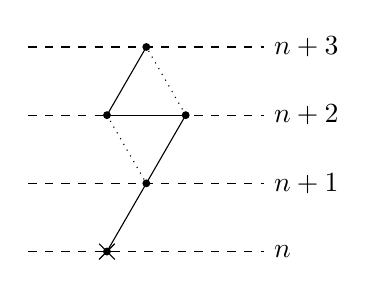
\begin{tikzpicture}
        \begin{scope}[shift=(0 : 0.0)]
          \draw (-0.1,-0.1) -- (0.1,0.1);
          \draw (0.1,-0.1) -- (-0.1,0.1);
          \draw (0 : 0.0) -- (60 : 1.0);
        \end{scope}
      \draw [dashed] (-1.0, 0.0) -- (2.0, 0.0);
      \fill (2.0, 0.0) node [right] {$n$};
      \draw [dashed] (-1.0, 0.866) -- (2.0, 0.866);
      \fill (2.0, 0.866) node [right] {$n+1$};
      \draw [dashed] (-1.0, 1.732) -- (2.0, 1.732);
      \fill (2.0, 1.732) node [right] {$n+2$};
      \draw [dashed] (-1.0, 2.598) -- (2.0, 2.598);
      \fill (2.0, 2.598) node [right] {$n+3$};
      \fill (0,0) circle [radius = 0.05];
      \begin{scope}[shift = (60 : 2.0)]
        \fill(0.0, 0.0) circle [radius = 0.05];
        \foreach \theta in {120, 180, 240}{
          \fill (0.0, 0.0) [transform canvas = {shift = (\theta : 1.0)}] circle [radius = 0.05];
        }
        \draw [dotted] (0 : 0.0) -- (120 : 1.0);
        \draw (0 : 0.0) -- (180 : 1.0);
        \draw (0 : 0.0) -- (240 : 1.0);
      \end{scope}
      \begin{scope}[shift = (60 : 1.0)]
        \begin{scope}[shift = (120 : 1.0)]
          \draw (0.0, 0.0) -- (60 : 1.0);
          \draw [dotted] (0.0, 0.0) -- (300 : 1.0);
        \end{scope}
      \end{scope}
    \end{tikzpicture}

    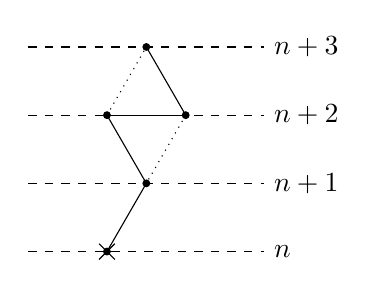
\begin{tikzpicture}
        \begin{scope}[shift=(0 : 0.0)]
          \draw (-0.1,-0.1) -- (0.1,0.1);
          \draw (0.1,-0.1) -- (-0.1,0.1);
          \draw (0 : 0.0) -- (60 : 1.0);
        \end{scope}
      \draw [dashed] (-1.0, 0.0) -- (2.0, 0.0);
      \fill (2.0, 0.0) node [right] {$n$};
      \draw [dashed] (-1.0, 0.866) -- (2.0, 0.866);
      \fill (2.0, 0.866) node [right] {$n+1$};
      \draw [dashed] (-1.0, 1.732) -- (2.0, 1.732);
      \fill (2.0, 1.732) node [right] {$n+2$};
      \draw [dashed] (-1.0, 2.598) -- (2.0, 2.598);
      \fill (2.0, 2.598) node [right] {$n+3$};
      \fill (0,0) circle [radius = 0.05];
      \begin{scope}[shift = (60 : 2.0)]
        \fill(0.0, 0.0) circle [radius = 0.05];
        \foreach \theta in {120, 180, 240}{
          \fill (0.0, 0.0) [transform canvas = {shift = (\theta : 1.0)}] circle [radius = 0.05];
        }
        \draw (0 : 0.0) -- (120 : 1.0);
        \draw (0 : 0.0) -- (180 : 1.0);
        \draw [dotted] (0 : 0.0) -- (240 : 1.0);
      \end{scope}
      \begin{scope}[shift = (60 : 1.0)]
        \begin{scope}[shift = (120 : 1.0)]
          \draw [dotted] (0.0, 0.0) -- (60 : 1.0);
          \draw (0.0, 0.0) -- (300 : 1.0);
        \end{scope}
      \end{scope}
    \end{tikzpicture}
    \end{tabular}
    \caption{}
    \label{fig:afterzigzag}
  \end{center}
\end{figure}

 If they form three bonds once, such as Fig.~\ref{fig:afterline}, the system would need three bonds forever to be deterministic. This becomes nondeterministic finally, such as in Fig.~\ref{fig:hexcorner}, when it reaches a corner of $\hexagon_p^n$. 
 %Therefore, the first fixed bead on a side of an equilateral hexagon with a radius of $n+1$ has to make a hydrogen bond with a molecule on a side of an equilateral hexagon with a radius of $n$.

\begin{figure}
  \begin{center}
  \begin{tabular}{cc}
    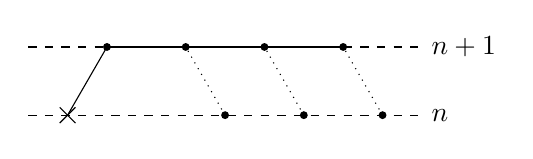
\begin{tikzpicture}
      \begin{scope}[shift=(0 : 0.0)]
        \draw (-0.1,-0.1) -- (0.1,0.1);
        \draw (0.1,-0.1) -- (-0.1,0.1);
        \draw (0 : 0.0) -- (60 : 1.0);
      \end{scope}
      \draw [dashed] (-0.5, 0.0) -- (4.5, 0.0);
      \fill (4.5, 0.0) node [right] {$n$};
      \draw [dashed] (-0.5, 0.866) -- (4.5, 0.866);
      \fill (4.5, 0.866) node [right] {$n+1$};
      \fill (2.0, 0.0) circle [radius = 0.05];
      \fill (3.0, 0.0) circle [radius = 0.05];
      \fill (4.0, 0.0) circle [radius = 0.05];
      \begin{scope}[shift = (60 : 1.0)]
        \fill (0.0, 0.0) circle [radius = 0.05];
        \fill (1.0, 0.0) circle [radius = 0.05];
        \fill (2.0, 0.0) circle [radius = 0.05];
        \fill (3.0, 0.0) circle [radius = 0.05];
        \draw (0.0, 0.0) -- (3.0, 0.0);
      \end{scope}
      \begin{scope}[shift = (0 : 2.0)]
        \draw [dotted] (0 : 0.0) -- (120 : 1.0);
      \end{scope}
      \begin{scope}[shift = (0 : 3.0)]
        \draw [dotted] (0 : 0.0) -- (120 : 1.0);
      \end{scope}
      \begin{scope}[shift = (0 : 4.0)]
        \draw [dotted] (0 : 0.0) -- (120 : 1.0);
      \end{scope}
    \end{tikzpicture}

    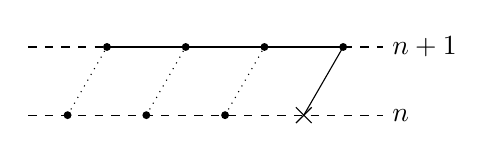
\begin{tikzpicture}
      \begin{scope}[shift=(0 : 0.0)]
        \draw (-0.1,-0.1) -- (0.1,0.1);
        \draw (0.1,-0.1) -- (-0.1,0.1);
        \draw (0 : 0.0) -- (60 : 1.0);
      \end{scope}
      \draw [dashed] (-3.5, 0.0) -- (1.0, 0.0);
      \fill (1.0, 0.0) node [right] {$n$};
      \draw [dashed] (-3.5, 0.866) -- (1.0, 0.866);
      \fill (1.0, 0.866) node [right] {$n+1$};
      \fill (-1.0, 0.0) circle [radius = 0.05];
      \fill (-2.0, 0.0) circle [radius = 0.05];
      \fill (-3.0, 0.0) circle [radius = 0.05];
      \begin{scope}[shift = (60 : 1.0)]
        \fill (0.0, 0.0) circle [radius = 0.05];
        \fill (-1.0, 0.0) circle [radius = 0.05];
        \fill (-2.0, 0.0) circle [radius = 0.05];
        \fill (-3.0, 0.0) circle [radius = 0.05];
        \draw (0.0, 0.0) -- (-3.0, 0.0);
      \end{scope}
      \begin{scope}[shift = (0 : -1.0)]
        \draw [dotted] (0 : 0.0) -- (60 : 1.0);
      \end{scope}
      \begin{scope}[shift = (0 : -2.0)]
        \draw [dotted] (0 : 0.0) -- (60 : 1.0);
      \end{scope}
      \begin{scope}[shift = (0 : -3.0)]
        \draw [dotted] (0 : 0.0) -- (60 : 1.0);
      \end{scope}
    \end{tikzpicture}
    \end{tabular}
    \caption{}
    \label{fig:afterline}
  \end{center}
\end{figure}

Accordingly, it is Fig.~\ref{fig:firstout} when a first bead is fixed on a side of an equilateral hexagon with a radius of $n+1$.

\begin{figure}
  \begin{center}
    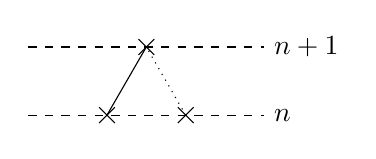
\begin{tikzpicture}
      \draw [dashed] (-1.0, 0.0) -- (2.0, 0.0);
      \fill (2.0, 0.0) node [right] {$n$};
      \draw [dashed] (-1.0, 0.866) -- (2.0, 0.866);
      \fill (2.0, 0.866) node [right] {$n+1$};
      \begin{scope}[shift=(0 : 0.0)]
        \draw (-0.1,-0.1) -- (0.1,0.1);
        \draw (0.1,-0.1) -- (-0.1,0.1);
        \draw (0 : 0.0) -- (60 : 1.0);
      \end{scope}
      \begin{scope}[shift=(60 : 1.0)]
        \draw (-0.1,-0.1) -- (0.1,0.1);
        \draw (0.1,-0.1) -- (-0.1,0.1);
      \end{scope}
      \begin{scope}[shift=(0 : 1.0)]
        \draw (-0.1,-0.1) -- (0.1,0.1);
        \draw (0.1,-0.1) -- (-0.1,0.1);
        \draw [dotted] (0 : 0.0) -- (120 : 1.0);
      \end{scope}
    \end{tikzpicture}
    \caption{}
    \label{fig:firstout}
  \end{center}
\end{figure}

%It has to be a right or left figure in Fig.6. when the first bead fixed on a side of an equilateral hexagon with a radius of $n+1$ make a hydrogen bond with a bead on a side of an equilateral hexagon with a radius of $n$. Fig.6. becomes nondeterministic finally, such as in Fig.7., when it reaches a corner of an equilateral hexagon. It is clear that all beads on a side of an equilateral hexagon with a radius of $n+1$ has to make a hydrogen bond with a bead on a side of an equilateral hexagon with a radius of $n$.  It is impossible to fix molecules on a side of an equilateral hexagon with a radius of $n+2$ and determine the only structure when there are only beads which are able to make a hydrogen bond in an equilateral hexagon with a radius of $n$.



%\section{Case of delay $1$}\label{sect:delay1}

\section{Upper bounds for determinisitc unary oritatami systems at delay 1 or arity 1}\label{sect:upper}





In this section, we consider Problem~\ref{prob:det_unary_length} at delay 1. Our result, cases of arity 1 and 3 can only yield finite structures of size $O (n)$, and cases of arity 4 and more can only yield finite structures which is size of $O (n^2)$, and a case of arity 2 can yield infinite structures but they are only the zig-zag conformation shown in Fig.~\ref{TTT_zigzag}. 

%In this section, we prove that unary oritatami system can form infinitely at delay 1 and arity 2 deterministically and moreover that the only infinite conformations which its oritatami system can yield is only the zig-zag conformation shown in Fig.\ref{TTT_zigzag}. 


Let $\Xi = (\Sigma, R, \delta, \alpha, \sigma, w)$ be a deterministic oritatami system of delay 1. 
For $i \geq 0$ let $C_i$ be the unique elongation of $\sigma$ by $w[1..i]$, that is, foldable by $\Xi$. Hence $C_0 = \sigma$.

\begin{comment}
\begin{figure}
  \begin{center}
    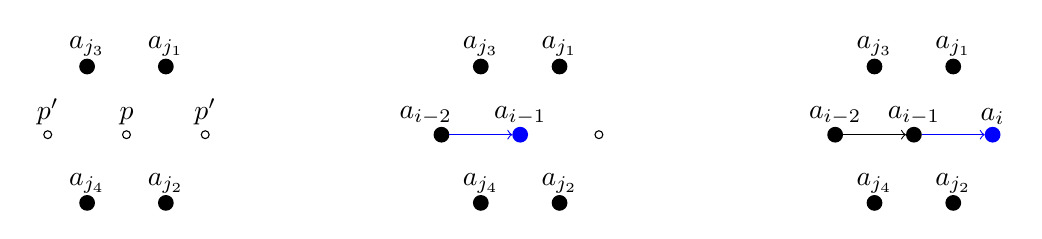
\begin{tikzpicture}
      \draw (0:0) circle [radius=0.05];
      \draw (0:1) circle [radius=0.05];
      \draw (180:1) circle [radius=0.05];
      \node[above] at (0:1) { $p^\prime$ };
      \node[above] at (0:0) { $p$ };
      \node[above] at (180:1) { $p^\prime$ };
      
      \fill (60 : 1) circle [radius=0.1];
      \fill (-60 : 1) circle [radius=0.1];
      \fill (120 : 1) circle [radius=0.1];
      \fill (-120 : 1) circle [radius=0.1];
      \node[above] at (60 :1) { $a_{j_1}$ };
      \node[above] at (-60 :1) { $a_{j_2}$ };
      \node[above] at (120 :1) { $a_{j_3}$ };
      \node[above] at (-120 :1) { $a_{j_4}$ };
      
      \begin{scope}[shift=(0:5)]
        \fill[blue] (0:0) circle [radius=0.1];
        \draw (0:1) circle [radius=0.05];
        \fill (180:1) circle [radius=0.1];
        \node[above] at (180:1.2) { $a_{i-2}$ };
        \node[above] at (0:0) { $a_{i-1}$ };
        \draw[->, blue] (180:0.9) -- (180:0.1);
        
        \fill (60 : 1) circle [radius=0.1];
        \fill (-60 : 1) circle [radius=0.1];
        \fill (120 : 1) circle [radius=0.1];
        \fill (-120 : 1) circle [radius=0.1];
        \node[above] at (60 :1) { $a_{j_1}$ };
        \node[above] at (-60 :1) { $a_{j_2}$ };
        \node[above] at (120 :1) { $a_{j_3}$ };
        \node[above] at (-120 :1) { $a_{j_4}$ };
      \end{scope}
      \begin{scope}[shift=(0:10)]
        \fill (0:0) circle [radius=0.1];
        \fill[blue] (0:1) circle [radius=0.1];
        \fill (180:1) circle [radius=0.1];
        \node[above] at (180:1) { $a_{i-2}$ };
        \node[above] at (0:0) { $a_{i-1}$ };
        \node[above] at (0:1) { $a_i$ };
        \draw[->] (180:0.9) -- (180:0.1);
        \draw[->,blue] (0:0.1) -- (0:0.9);
        
        \fill (60 : 1) circle [radius=0.1];
        \fill (-60 : 1) circle [radius=0.1];
        \fill (120 : 1) circle [radius=0.1];
        \fill (-120 : 1) circle [radius=0.1];
        \node[above] at (60 :1) { $a_{j_1}$ };
        \node[above] at (-60 :1) { $a_{j_2}$ };
        \node[above] at (120 :1) { $a_{j_3}$ };
        \node[above] at (-120 :1) { $a_{j_4}$ };
      \end{scope}
    \end{tikzpicture} 
    \caption{Through a tunnel section}
    \label{TTT_tunnel_intro}
  \end{center}
\end{figure}
\end{comment}

\begin{figure}[tb]
  \begin{center}
    \begin{tabular}{ccc}
      
      \begin{minipage}{0.3\hsize}
        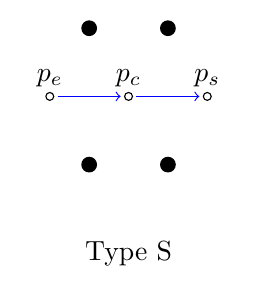
\begin{tikzpicture}
          \begin{scope}[xshift=2cm, yshift=2cm]
          
            \draw[white] (60:1) -- (0:0);
            \draw[white] (-60:1) -- (0:0);
            \draw(0,0) circle [radius=0.05];
            \node[above] at (0,0) {$p_c$};
            \node[above] at (180:1) {$p_e$};
            \node[above] at (0:1) {$p_s$};

            \foreach \theta in {0,180}{
              \draw[transform canvas={shift=(\theta:1)}](0,0) circle [radius=0.05];
            }
            
            \foreach \theta in {60,-60,120,-120}{
              \fill[transform canvas={shift=(\theta:1)}](0,0) circle [radius=0.1];
            }
          \draw[->, blue] (-0.9, 0) -- (-0.1, 0);
          \draw[->, blue] (0.1, 0) -- (0.9, 0);
          \end{scope}
          

          \node at (2,0) {Type S};
        \end{tikzpicture}
      \end{minipage}

      \begin{minipage}{0.3\hsize}
        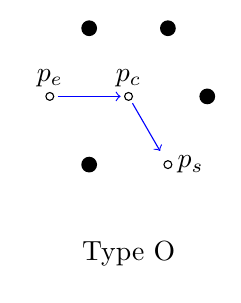
\begin{tikzpicture}

          \begin{scope}[xshift=2cm, yshift=2cm]
          
            \draw[white] (60:1) -- (0:0);
            \draw[white] (-60:1) -- (0:0);
            \draw(0,0) circle [radius=0.05];
            \node[above] at (0,0) {$p_c$};
            \node[above] at (180:1) {$p_e$};
            \node[right] at (-60:1) {$p_s$};

            \foreach \theta in {-60,180}{
              \draw[transform canvas={shift=(\theta:1)}](0,0) circle [radius=0.05];
            }
            
            \foreach \theta in {0,60,120,-120}{
 	            \fill[transform canvas={shift=(\theta:1)}](0,0) circle [radius=0.1];
            }
          \draw[->, blue] (-0.9, 0) -- (-0.1, 0);
          \draw[->, blue] (0,0)++(300:0.1) -- (300:0.8);
          \end{scope}

          \node at (2,0) {Type O};
        \end{tikzpicture}
      \end{minipage}

      \begin{minipage}{0.3\hsize}
        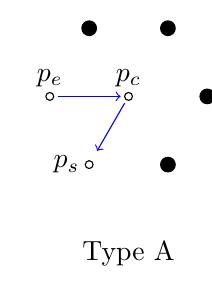
\begin{tikzpicture}

          \begin{scope}[xshift=2cm, yshift=2cm]
            \draw[white] (60:1) -- (0:0);
            \draw[white] (-60:1) -- (0:0);
            \draw(0,0) circle [radius=0.05];
            \node[above] at (0,0) {$p_c$};
            \node[above] at (180:1) {$p_e$};
            \node[left] at (-120:1) {$p_s$};

            \foreach \theta in {-120,180}{
              \draw[transform canvas={shift=(\theta:1)}](0,0) circle [radius=0.05];
            }
            
            \foreach \theta in {0,60,-60,120}{
              \fill[transform canvas={shift=(\theta:1)}](0,0) circle [radius=0.1];
            }
          \draw[->, blue] (-0.9, 0) -- (-0.1, 0);
          \draw[->, blue] (0,0)++(240:0.1) -- (240:0.8);
          \end{scope}

          \node at (2,0) {Type A};
        \end{tikzpicture}
      \end{minipage}
      
    \end{tabular}
    \caption{Tunnel sections of all possible three types: straight (Type S), obtuse turn (Type O), and acute turn (Type A).}
    \label{fig:TTT_tunnel}
  \end{center}
\end{figure}

At delay 1, a bead cannot collaborate with its successors in order to stabilize itself. 
In fact, there are just two ways for a bead to get stabilized at delay 1 (or the bead has no place to be stabilized around so that the system halts), as observed in \cite{DHOPRSST2018}. 
One is to be bound to another bead and the other is through a 1-in-1-out structure called the tunnel section. 
See Fig.~\ref{fig:TTT_tunnel}. 
A \textit{tunnel section} consists of one free point $p_c$ and four beads that occupy four neighbors of $p_c$. 
In order for an oritatami system to stabilize the bead $w[i]$ at the central point $p_c$, its predecessor $w[i-1]$ must be put at one of the two free neighbors of $p$. 
Thus, at the stabilization of $w[i]$, only one neighbor of $p$ is left free so that the successor $w[i+1]$ is to be stabilized there, even without being bound. 
In this case, the point $p_e$ where $w[i-1]$ is stabilized is considered to be an \textit{entrance of the tunnel section} and the point $p_s$ where $w[i+1]$ is stabilized is considered as its \textit{exit}. 
A \textit{tunnel} is a maximal set of tunnel sections whose central points form a path. 

The behavior of an oritatami system at delay 1 can be described by a sequence of $S$ of $b$ (bound), $t_s$ (straight tunnel section), $t_o$ (obtuse-turn tunnel section), and $t_a$ (acute-turn tunnel section); priority is given to tunnel, that is, $S[i]$ is $t_s$ (resp.~$t_o$, $t_a$) if the $i$-th bead of the system is stabilized not only by being bonded but also through a straight (resp. obtuse-turn, acute-turn) tunnel section. 
Let us introduce $t$ as a wildcard for $t_s$, $t_o$, and $t_a$. 
We also let $S$ take the value $\blacksquare$ for halt (due to the lack of free neighbors). 

%If a bead is stabilized through a tunnel section, then it can provide some bonds. Let us consider bonds of $C_i$. $C_i$ is represented $C = (W,P,H)$ where $|W| = i + n$ $C_i$ contains $\alpha \cdot (i + n) - 2|H|$ bonds because $C_i$ consists of $i + n$ beads and a bead has just $\alpha$ bonds and then $2 |H|$ of the those bonds are already used. However, even if a bead has an available bond, $w[j]$ $(j > i)$ might not be able to use this bond because the bond has possibility that it is blocked by transcripts $w[i+1..j-1]$. Number of $binding\ capabilities$ does not contain that case so that it is at most $\alpha \cdot (i + n) - 2|H|$.

%We say that point $p$ is reachable from a conformation $C$ if there exists a directed path $P^\prime$ from the last point of $C$ that does not cross the path of $C$. 
We say that a neighbor of a point $p$ is reachable from a conformation $C$ if there exists an elongation of $C$ in which a bead occupies the neighbor and it binds with a bead at $p$. 
Taking this reachability into account, we define the \textit{binding capability} of a conformation as the number of free bonds of its beads available geometrically for elongations of $C$.
It is defined formally as follows: 

\begin{definition}[Binding Capability]
Let $\alpha$ be an arity and $C = (P,w,H)$ be a conformation of arity at most $\alpha$.
Let $H_k = H \cap \{ (i,j) \mid \mbox{$i=k$ or $j=k$} \}$. 
Moreover, let $R_k$ be a set of neighbors of the point $P[k]$ that are free and reachable from $C$.
The binding capability of $C$ at arity $\alpha$, denoted by $\#bc_\alpha(C)$, is defined by $\sum^{|w|}_{k=1} \min \{\alpha-|H_k|, |R_k|\}$.
The subscript $\alpha$ is omitted whenever it is clear from context. 
\end{definition}
%
Observe one almost-trivial but important fact that a bead inside a tunnel does not increase the binding capability. 
This is because for such a bead $w[k]$, $|R_k| = 0$. 

We now prove that in ``almost all'' tunnels is a troll domiciled and robs the transcript of binding capability (the original story is from \cite{Pratchett1992}). 
Originally, we tried to find a troll in every tunnel but failed; a troll seems to dislike the very first bead $w[1]$, or its property that only $\alpha$+1 beads around may take all hands of $w[1]$ thanks to the absence of its predecessor; any other bead must be surrounded by at least $\alpha+2$ beads in order to be free from free hand because a bead cannot bind with its predecessor or successor. 
We call a bead \textit{singular} if it is surrounded by only $\alpha+1$ beads but forms $\alpha$ bonds. 
Any bead but $w[1]$ can be singular because of their predecessor and successor. 
A tunnel is \textit{singular} if its entrance or exit is next to $w[1]$ that is singular. 
There can be at most 3 tunnels around one bead so that no more than 3 tunnels can be singular. 
A singular tunnel will be denoted with the superscript $\times$ like $t_s^\times$ or $t^\times$. 
In contrast, the notation without $\times$ such as $t_s$ and $t$ shall imply their non-singularity. 



%remark 

\begin{theorem}[Tunnel Troll Theorem]
\label{TTT}
Let $\Xi$ be a deterministic unary oritatami system of delay $\delta = 1$. The following statements hold.
\begin{enumerate}
\item At arity $\alpha \geq 3$, if $S[i] = t$ (i.e. the tunnel that stabilizes $w[i]$ is not singular) and $S[i+1] \neq \blacksquare$, then $\#bc(C_{i-1}) > \#bc(C_i)$.
\item At arity $\alpha = 2$, if $m$ is the number of occurrences of $bt$ as a factor in $S[1..k]$ for an index $k$, then $\#bc(C_{0}) - m \geq \#bc(C_{k})$.
\end{enumerate}
\end{theorem}

In order to prove this theorem, we use the following three lemmas.
%Let us introduce some lemmas for proving Tunnel Troll Theorem.

%%%%%%%%%%%%%%%%%%%%%%%%%%%%%%%%%%%%%%%%%%%%%%%%%%%%

\begin{lemma}
\label{TTT_entrance_Tab}
Let $\Xi$ be a deterministic unary oritatami system at delay $\delta = 1$ and arity $\alpha =2$. 
Assume $\Xi$ stabilizes the transcript until $w[i-1]$. If $S[i+1] = b$ and $S[i+2] \in \{ t_s, t_o \} $, then $\#bc(C_{i-1}) > \#bc(C_{i})$.
\end{lemma}

\begin{proof}%[lemma \ref{TTT_entrance_Tab}]
See Fig.\ref{TTT_tunnel_direction}.
$S[i+2] \in \{ t_s, t_o \} $ means that $w[i+2]$ is stabilized by a tunnel section of type S or O.
Thus,  its predecessor $w[i+1]$ must be inside the tunnel section, that is, $n_1$ and $n_2$ must be occupied.
Free bonds of $w[i]$, if any, cannot be used in future by another bead $w[j]$ because otherwise the part of transcript $w[i..j]$ and the bond between $w[i]$ and $w[j]$ would form a closed curve and the curve would cross the path of $C_{i-1}$ between $n_1$ and $n_2$, contradiction.
%Binding capabilities that $w[i]$ supplies are inactive according to Jordan curve theorem on $n_1$, $n_2$, and $w[i]$.
Therefore, if $w[i]$ forms a bond at its stabilization $\#bc(C_{i-1}) > \#bc(C_{i})$ holds.
We now prove that $w[i]$ must form a bond.


Suppose $w[i]$ were stabilized without any bond, that is, by a tunnel.
For that the two points that are a neighbor of both $w[i-1]$ and $w[i]$ must be occupied already.
In addition, at least one of the neighbors of $w[i]$ must be free because $S[i+1] = b$.
Thus, only the case to be considered is Fig.~\ref{TTT_tunnel_direction} (middle) with $n_5$ being occupied (that is, $n_4$ is free).
In this case, before $w[i]$ is stabilized, at lest three neighbors of $n_2$ were free and hence, a bead at $n_2$ was provided with one free bond and could form a bond with $w[i]$. \qed

\end{proof}

\begin{figure}[tb]
  \begin{center}
    \begin{tabular}{ccc}
    
    
      \begin{minipage}{0.3\hsize}
      \centering
        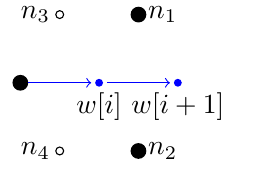
\begin{tikzpicture}
        \draw[->, white] (0:0)--(-120:1);
	 \draw[->,white] (120:0.8)--(120:0.1);%for adjustment
          
            \fill[blue] (0,0) circle [radius=0.05];
            \node[below] at (0,0) {$w[i]$};
            \node[below] at (0:1) {$w[i+1]$};

            \foreach \theta in {0}{
              \fill[transform canvas={shift=(\theta:1)},blue](0,0) circle [radius=0.05];
            }
            
            \foreach \theta in {60,-60,180}{
              \fill[transform canvas={shift=(\theta:1)}](0,0) circle [radius=0.1];
            }

            \foreach \theta in {120,-120}{
              \draw[transform canvas={shift=(\theta:1)}](0,0) circle [radius=0.05];
            }
            
            \draw[->, blue] (180:0.9)--(180:0.1);
            \draw[->, blue] (0:0.1)--(0:0.9);

            \node[transform canvas={shift=(60:1)},right] {$n_1$};
            \node[transform canvas={shift=(-60:1)},right] {$n_2$};
            \node[transform canvas={shift=(120:1)},left] {$n_3$};
            \node[transform canvas={shift=(-120:1)},left] {$n_4$};


         % \node at (0,-2) {$t_{0}$};
        \end{tikzpicture}
      \end{minipage}

      

      \begin{minipage}{0.3\hsize}
      \centering
        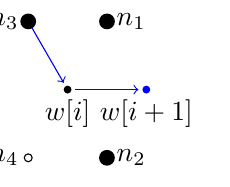
\begin{tikzpicture}
	\draw[->, white] (0:0)--(-120:1);
            \fill(0,0) circle [radius=0.05];
            \node[below] at (0,0) {$w[i]$};
            \node[below] at (0:1) {$w[i+1]$};

            \foreach \theta in {0}{
              \fill[transform canvas={shift=(\theta:1)},blue](0,0) circle [radius=0.05];
            }
            
            \foreach \theta in {60,-60,120}{
              \fill[transform canvas={shift=(\theta:1)}](0,0) circle [radius=0.1];
            }

            \foreach \theta in {180,-120}{
              \draw[transform canvas={shift=(\theta:1)}](0,0) circle [radius=0.05];
            }
            
            \draw[->, blue] (120:0.9)--(120:0.1);
            \draw[->, blue] (0:0.1)--(0:0.9);

            \node[transform canvas={shift=(60:1)},right] {$n_1$};
            \node[transform canvas={shift=(-60:1)},right] {$n_2$};
            \node[transform canvas={shift=(120:1)},left] {$n_3$};
            \node[transform canvas={shift=(-120:1)},left] {$n_4$};
            \node[transform canvas={shift=(180:1)},left] {$n_5$};

          %\node at (0,-2) {$t_{\pm 60}$};
        \end{tikzpicture}
      \end{minipage}

      \begin{minipage}{0.3\hsize}
      \centering
        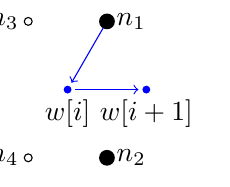
\begin{tikzpicture}
        \draw[->, white] (0:0)--(-120:1);
            \fill[blue](0,0) circle [radius=0.05];
            \node[below] at (0,0) {$w[i]$};
            \node[below] at (0:1) {$w[i+1]$};

            \foreach \theta in {0}{
              \fill[transform canvas={shift=(\theta:1)}, blue](0,0) circle [radius=0.05];
            }
            
            \foreach \theta in {60,-60}{
              \fill[transform canvas={shift=(\theta:1)}](0,0) circle [radius=0.1];
            }

            \foreach \theta in {180,-120,120}{
              \draw[transform canvas={shift=(\theta:1)}](0,0) circle [radius=0.05];
            }
            
            \draw[->, blue] (60:0.9)--(60:0.1);
            \draw[->, blue] (0:0.1)--(0:0.9);

            %\node[transform canvas={shift=(0:1)},below] {$n_0$};
            \node[transform canvas={shift=(60:1)},right] {$n_1$};
            \node[transform canvas={shift=(-60:1)},right] {$n_2$};
            \node[transform canvas={shift=(120:1)},left] {$n_3$};
            \node[transform canvas={shift=(-120:1)},left] {$n_4$};
            \node[transform canvas={shift=(180:1)},left] {$n_5$};

         % \node at (0,-2) {$t_{\pm 120}$};
        \end{tikzpicture}
      \end{minipage}
      
    \end{tabular}
    \caption{The three ways to enter a tunnel: (Left) straight, (Middle) obtuse, (Right) acute. The bead $w[i]$ is stabilized at the entrance and $w[i+1]$ is stabilized inside.}
    \label{TTT_tunnel_direction}
  \end{center}
\end{figure}


%%%%%%%%%%%%%%%%%%%%%%%%%%%%%%%%%%%%%%%%%%%%%%%%%%%%

\begin{lemma}
\label{TTT_exit}
Let $\Xi$ be a deterministic unary oritatami system of delay $\delta = 1$ and arity $\alpha =2$.
%Let $w[i]$ be a bead which is stabilized at the exit of a tunnel.
If $S[i+1..j+1] = bt^{(j-i-1)}b$ for some $i,j$ with $i \leq j-2$ and $S[j] \in \{ t_s, t_o\}$, then $\#bc(C_{j-2}) \geq \#bc(C_j)$, and hence, $\#bc(C_{i}) \geq \#bc(C_j)$.
If $i \leq j-3$, then the second inequality is strengthened as $\#bc(C_{i}) > \#bc(C_{j})$.
%if we assume $\#bc(C_{i-2}) - \#bc(C_{i-1}) = a$, then $\#bc(C_{i}) - \#bc(C_{i-1}) \leq a$.
\end{lemma}

\begin{proof}%[Lemma~ \ref{TTT_exit}]
Since the binding capability never increases inside a tunnel, we just need to consider the exit of a tunnel.
See Fig.\ref{TTT_tunnel_exit}. 
At least one of points $n_1$ or $n_2$ must be free because otherwise $w[j]$ would be inside of a tunnel, that is, $S[j+1]$ would not be $b$.



Let $m$ be the number of bonds $w[j-1]$ forms, that is, $\#bc(C_{j-2}) - \#bc(C_{j-1}) = m$.
We claim $\#bc(C_{j}) - \#bc(C_{j-1}) \leq m$.
Indeed, if both $n_1$ and $n_2$ are free (see Fig.~\ref{TTT_tunnel_exit}), the predecessor $w[j-1]$ must be bound to both beads at $n_3$ and at $n_4$ because both of them still have a free hand.
Hence, $m \geq 2$.
Since $\#bc(C_{j}) - \#bc(C_{j-1})$ is less than the arity, this difference is at most $m$.

If $n_1$ is occupied, then $n_2$ is free.
The predecessor $w[j-1]$ must be bound $n_4$.
Hence,  $m \geq 1$.
The bead $w[j]$ can increase the binding capability at most by 1 because one of its free neighbors would, $n_0$ or $n_2$, is to be occupied by the successor $w[j+1]$.
Therefore, $\#bc(C_{j}) - \#bc(C_{j-1}) \leq m$.
  


Thus,$\#bc(C_{j-2}) \geq \#bc(C_j)$ , and hence, $\#bc(C_{i}) \geq \#bc(C_j)$.
If $i \leq j-3$, then the second inequality is strengthened as $\#bc(C_{i}) > \#bc(C_{j})$ because $S[i+1] = b$, that is, $\#bc(C_{i}) > \#bc(C_{i+1})$ and $\#bc(C_{i+1}) \geq \#bc(C_j)$. \qed


\end{proof}

\begin{figure}[tb]
  \centering
    \begin{tabular}{cc}
    \centering
      \begin{minipage}{0.45\linewidth}
      \centering
        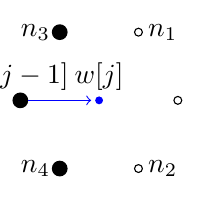
\begin{tikzpicture}
	\draw[white] (0:0) -- (120:1);
	\draw[white] (0:0) -- (-60:1);
	\draw[white] (0:0) -- (0:1);

            \fill[blue](0,0) circle [radius=0.05];
            \node[above] at (0,0) {$w[j]$};

            
            \foreach \theta in {120,-120,180}{
              \fill[transform canvas={shift=(\theta:1)}](0,0) circle [radius=0.1];
            }

            \foreach \theta in {0}{
              \draw[transform canvas={shift=(\theta:1)}](0,0) circle [radius=0.05];            }
            \draw (-60:1) circle [radius=0.05];
            \draw (60:1) circle [radius=0.05];

            \draw[->, blue] (180:0.9)--(180:0.1);



            \node[transform canvas={shift=(60:1)},right] {$n_1$};
            \node[transform canvas={shift=(-60:1)},right] {$n_2$};
            \node[transform canvas={shift=(120:1)},left] {$n_3$};
            \node[transform canvas={shift=(-120:1)},left] {$n_4$};
            \node[transform canvas={shift=(180:1)},above] {$w[j-1]$};

        \end{tikzpicture}
      \end{minipage}

      \begin{minipage}{0.45\linewidth}
      \centering
        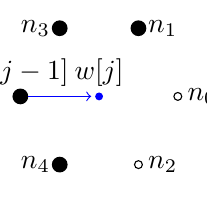
\begin{tikzpicture}

	\draw[white] (0:0) -- (120:1);
	\draw[white] (0:0) -- (-60:1);
	\draw[white] (0:0) -- (0:1);

            \fill[blue](0,0) circle [radius=0.05];
            \node[above] at (0,0) {$w[j]$};
            
            \foreach \theta in {120,-120,180,60}{
              \fill[transform canvas={shift=(\theta:1)}](0,0) circle [radius=0.1];
            }

            \foreach \theta in {0}{
              \draw[transform canvas={shift=(\theta:1)}](0,0) circle [radius=0.05];
            }
            \draw (-60:1) circle [radius=0.05];

            \draw[->, blue] (180:0.9)--(180:0.1);

            \node[transform canvas={shift=(0:1)},right] {$n_0$};
            \node[transform canvas={shift=(60:1)},right] {$n_1$};
            \node[transform canvas={shift=(-60:1)},right] {$n_2$};
            \node[transform canvas={shift=(120:1)},left] {$n_3$};
            \node[transform canvas={shift=(-120:1)},left] {$n_4$};
            \node[transform canvas={shift=(180:1)},above] {$w[j-1]$};

        \end{tikzpicture}
      \end{minipage}
    \end{tabular}
    \caption{Two kinds of exit of a tunnel: (Left) Both $n_1$ and $ n_2$ are free, (Right) One of $n_1$ and $n_2$ is occupied.}
    \label{TTT_tunnel_exit}
\end{figure}

%%%%%%%%%%%%%%%%%%%%%%%%%%%%%%%%%%%%%%%%%%%%%%%%%%%%


\begin{lemma}
\label{TTT_tunnelC_lemma}
Let $\Xi$ be a deterministic unary oritatami system of delay $\delta = 1$ and arity $\alpha = 2$.
If $S[i+2] = t_a$, the following statements hold.
\begin{enumerate}
\item If $w[i]$ forms at least one bond, $\#bc(C_{i-1}) > \#bc(C_{i+2})$.
\item If $w[i]$ does not consume any bond and $S[i] \in \{t_s, t_o \}$, $\#bc(C_{i-2}) > \#bc(C_{i+2})$.
\item If $w[i]$ does not consume any bond and $S[i] = t_a$, $\#bc(C_{i-3}) - 2 \geq \#bc(C_{i+2})$.
\end{enumerate}
%If there are indices $i,j$ such that $S[i..j+1]$ is either $bbt^{(j-i-1)}b$ and $S[i+2] = t_a$ or $bt^\ell bt^{j-i-1-\ell}b$ for some $\ell$ and $S[i+l+2] = t_a$, then $\#bc(C_{i-1}) > \#bc(C_j)$.
\end{lemma}

\begin{proof}

	We consider each statement. First we prove Statement 1.
	The bead $w[i+1]$ consumes one hand and provides nothing.
	If $w[i]$ forms two bonds, then even if $w[i+2]$ provides two free hands, $\#bc(C_{i-1}) > \#bc(C_{i+2})$.
	On the other hand, if it leaves a free hand, it will be used by $w[i+2]$, and hence, $w[i+2]$ does not increase the binding capability.
	Thus, $\#bc(C_{i-1}) > \#bc(C_{i+2})$.
	This argument actually work also for the case when $w[i]$ is stabilized rather by binding.
	
	Let us proceed to Statement 2.
	See Fig.~\ref{TTT_tunnelC_enter_usingBond}.
	Consider the case when $w[i]$ is stabilized by a tunnel section of type S or O.
	As prove in Lemma~\ref{TTT_exit}, $\#bc(C_{i-2}) \geq \#bc(C_{i})$.	The bead $w[i]$ leaves two free hand, it will be used by $w[i+2]$, and hence, $w[i+2]$ does not increase the binding capability.
	Thus, $\#bc(C_{i-2}) > \#bc(C_{i+2})$.
	This argument actually work also for the case when $w[i]$ is stabilized rather by binding.
	
	We finalize this proof by showing Statement 3.
	In order for $w[i]$ not to bind, $w[i-2]$ must have already used up its hands.
	The bead $w[i-1]$ consumes one hand and provides nothing.
	Thus,  $\#bc(C_{i-3}) - 1 \geq \#bc(C_{i})$.
	The bead $w[i+1]$ consumes one hand and provides nothing.
	Finally, $w[i+2]$ uses one hand of $w[i]$, and hence, does not increase the binding capability.
	Therefore, $\#bc(C_{i-3}) -2 \geq \#bc(C_{i+2})$.
	This argument actually works also for the case when $w[i]$ is stabilized rather by binding. \qed
\end{proof}

\begin{figure}[tb]
  \begin{center}
  \begin{tabular} {c c}
  \begin{minipage}{0.48\hsize}
  \centering
        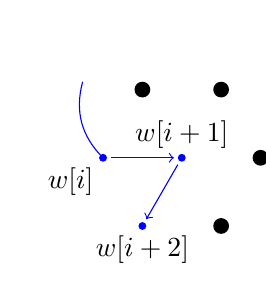
\begin{tikzpicture}
        \draw[->, white, shift=(180:1), shift=(120:1)] (120:0.9) -- (120:0.1);
          \foreach \theta in {60,-60,120,0}{
            \fill[transform canvas={shift=(\theta:1)}](0,0) circle [radius=0.1];
          }

          \fill[blue](180:1) circle [radius=0.05];
          \fill[blue](0:0) circle [radius=0.05];

          \draw[transform canvas={shift=(180:1)}, blue] (105:1) edge[bend right] (105:0);
          \draw[->, blue] (180:0.9) -- (180:0.1);
          \draw[->, blue] (-120:0.1) -- (-120:0.9);

          \node[below left] at (180:1) {$w[i]$};
          \node[above] at (0:0) {$w[i+1]$};
          \node[below] at (-120:1) {$w[i+2]$};
          \begin{scope}[shift=(-120:1)]
            \fill[blue](0,0) circle [radius=0.05];
            
          \end{scope}
        \end{tikzpicture}

	\end{minipage}
	
	\begin{minipage}{0.48\hsize}     
        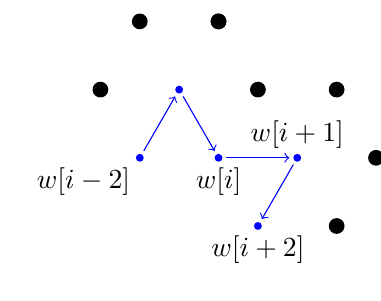
\begin{tikzpicture}
         \draw[->, white, shift=(180:1), shift=(120:1)] (120:0.9) -- (120:0.1);
          \foreach \theta in {60,-60,120,0}{
            \fill[transform canvas={shift=(\theta:1)}](0,0) circle [radius=0.1];
          }
          
          \foreach \theta in {60,60,120,180}{
            \fill[transform canvas={shift=(\theta:1)}, shift=(180:1)](120:1) circle [radius=0.1];
          }

          \fill[blue](180:1) circle [radius=0.05];
          \fill[blue](0:0) circle [radius=0.05];
          \fill[blue, shift=(180:1), shift=(120:1)](0:0) circle [radius=0.05];
          \fill[blue, shift=(180:1), shift=(120:1)](-120:1) circle [radius=0.05];

          
          \draw[->, blue] (180:0.9) -- (180:0.1);
          \draw[->, blue] (-120:0.1) -- (-120:0.9);
          \draw[->, blue, shift=(180:1), shift=(120:1)] (-60:0.1) -- (-60:0.9);
           \draw[->, blue, shift=(180:1), shift=(120:1)] (-120:0.9) -- (-120:0.1);

          \node[below] at (180:1) {$w[i]$};
          \node[above] at (0:0) {$w[i+1]$};
          \node[below] at (-120:1) {$w[i+2]$};
          \node[below left] at (-180:2) {$w[i-2]$};

          \begin{scope}[shift=(-120:1)]
            \fill[blue](0,0) circle [radius=0.05];
            
          \end{scope}
        \end{tikzpicture}
        \end{minipage}
        \end{tabular}
    \caption{The bead $w[i+2]$ is stabilized by a tunnel of type A. (Right) Moreover $S[i] = t_a$.}
    \label{TTT_tunnelC_enter_usingBond}
  \end{center}
\end{figure}


%%%%%%%%%%%%%%%%%%%%%%%%%%%%%%%%%%%%%%%%%%%%%%%%%%%%
%%
%%%%
%%%%%%
%%%%%%%%
%%%%%%%%%%%%%%%%%%%%%%%%%%%%%%%%%%%%%%%%%%%%%%%%%%%%

%Each bead in the transcript is bound either inside a tunnel or outside. If a bead is stabilized inside a tunnel, 
%then it has at most one free neighbor, and hence its successor it to be stabilized there.
%Moreover, if a bead is stabilized outside a tunnel, then its position is either an entrance of a tunnel or not.
%
%Tunnel sections have three possible shapes up to symmetry : straight($S$), obtuse($O$) and acute($A$) turn (Fig. \ref{fig:TTT_tunnel}), and we will consider each of those. 


%\begin{lemma}
%\label{TTT_neighbor_lemma}
%For unary transcripts at $\delta = 1$, if a bead has no free hand, then at least $\alpha + 2$ of its neighbors have to be occpied.
%\end{lemma}

Now we are ready to prove the Tunnel Troll Theorem.

\begin{proof}%{Proof of Tunnel Troll Theorem}
Let us first consider cases of $\delta \geq 3, \alpha = 1$. 
See Fig.~\ref{TTT_tunnel_exit}. Consider the stabilization of $w[i]$. 
This bead $w[i]$, once stabilized, shares two neighbors with its predecessor $w[i-1]$, which are denoted by $n_3, n_4$. 
Both of them have been already occupied because $S[i] = t$. 

Since $S[i+1] \neq \blacksquare$, at least one of the other three neighbors, denoted by $n_0, n_1, n_2$, must be free. 
Assume that in the neighborhood of $w[i]$, there are two beads with one free neighbor even after $w[i]$ is stabilized. 
Before the stabilization of $w[i]$, such a bead had two free neighbors, and hence, is provided with at least one free bond. 
Thus, $w[i]$ is to be bonded to these two beads, and it decreases the binding capability by at least 1. 
It now suffices to check that this assumption holds no matter how $n_0, n_1, n_2$ are occupied as long as at least one of them is left free. 

Next, we consider the case of $\delta = 2, \alpha = 1$. We assume there are indices $i$, $j$ such that $S[i+1..j+1] = bt^{(j-i-1)}b$.
If $S[i+2]$ is $ t_s$ or  $t_o$, then Lemma~\ref{TTT_entrance_Tab} implies $\#bc(C_{i-1}) > \#bc(C_{i})$ and  Lemma~\ref{TTT_exit} implies $\#bc(C_{i}) \geq \#bc(C_{j})$.
Thus, binding capability decreases by 1 per a factor $bt_s$ or $bt_o$.


%All $S[i+3..j]$ do not contain $t_a$; otherwise $S[i+4..j+1]$ contain $\blacksquare$.
%Therefore, $S[i+2] = t_a$.
Now, we assume $S[i+2] = t_a$.
Then, we have to make sure that one troll is not double-counted.
If $w[i]$ forms a bond, Lemmas~\ref{TTT_exit} and \ref{TTT_tunnelC_lemma} imply that binding capability decreases through this tunnel.

Assume $w[i]$ forms no bond.
If $S[i] \in \{t_s, t_o\}$, Lemmas~\ref{TTT_exit} and \ref{TTT_tunnelC_lemma} imply $\#bc(C_{i-2}) > \#bc(C_{i+2})$.
Observe that the bead $w[i-1]$ is at the entrance of the previous tunnel or inside.
It is when a bead is stabilized at the entrance of a tunnel that the troll of the tunnel decreases binding capability.
Thus, the inequality does not rely on the troll of previous tunnel.
If $S[i] = t_a$, Lemma~\ref{TTT_tunnelC_lemma} implies $\#bc(C_{i-3}) - 2 \geq \#bc(C_{i+2})$.
%The previous tunnel must be indeed a tunnel section of type A (see Fig.~\ref{TTT_tunnelC_enter_usingBond}).
This inequality involves two tunnels but its difference 2 enables us to consider that binding capability decreases by 1 through this tunnel. \qed
\end{proof}





%%%%%%%%%%%%%%%%%%%%%%%%%%%%%%%%%%%%%%%%%%%%%%%%%%%%%%%%%
%/////////////////////////////////////////////////
%%%%%%%%%%%%%%%%%%%%%%%%%%%%%%%%%%%%%%%%%%%%%%%%%%%%%%%%%


\subsection{Upper bounds on the length of conformation foldable deterministically at delay $\delta = 1$.}


\begin{theorem}[$\delta = 1, \alpha = 4$]
Let $\Xi$ be a deterministic unary oritatami system of $\delta = 1, \alpha = 4$. It can yield only finite conformation of length $3n^2  + 3n + 1$.
\end{theorem}

\begin{proof}
Consider the moment when a bead $b$ is stabilized outside $\hexagon_O^n$ for the first time. 
See Fig.~\ref{TTT_a4_first}.
There is only one bead available to stabilize $b$ there, which is $b_1$. 
In order for $b$ to avoid nondeterminism, hence, none of the beads around should not attract $b$. 

The point $p_1$ must be empty because a bead there would have at least two free neighbors and hence is provided with a free hand. 
If there is a bead at $p_2$, $n$ must be at least 2 so that the bead is not singular. 
Since $p_1$ is empty, this bead has at least one free hand, a contradiction. 
Thus, $p_2$ must be also empty. 
In the same way, we can easily show that the point $p_3$ must not be occupied by a non-singular bead. 
Suppose $p_3 = O$. 
The point $p_4$ must not be empty; otherwise the singular bead, at $O$, would have a free hand. 
However, then a bead at $p_4$ would be provided with a free hand, a contradiction. 
\qed
\end{proof}

\begin{figure}[tb]
 \centering
    \begin{tikzpicture}

	\fill (0,0) circle [radius=0.1];
        \fill[blue] (60:1) circle [radius=0.05];
        \fill (0:1) circle [radius=0.1];
      
      \draw[dashed] (180:2) -- (0:2);
      \draw[dashed, shift=(60:1)] (180:2.5) -- (0:1.5);
      \draw[->, blue] (60:0.1) -- (60:0.9);

	\node[above] at (180:1) {$p_1$};
	\node[left] at (-120:1) {$p_2$};
	\node[left, shift=(-120:1)] at (-60:1) {$p_3$};
	\node[right] at (-60:1) {$p_4$};

	\draw (180:1) circle [radius=0.05];
	\draw (-120:1) circle [radius=0.05];
	\draw (-60:1) circle [radius=0.05];
	\draw[shift=(-120:1)] (-60:1) circle [radius=0.05];

	\node at (0:2.5) {$n$};
	\node[shift=(60:1)] at (0:2) {$n+1$};
    \end{tikzpicture}
    \caption{The first bead out of $\hexagon_{O}^n$}
    \label{TTT_a4_first}
\end{figure}


%%%%%%%%%%%%%%%%%%%%%%%%%%%%%%%%%%%%%%%%%%%%%%%%%%%%%%%%%


\begin{theorem}[$\delta = 1, \alpha = 3$]
Let $\Xi$ be a deterministic unary oritatami system of $\delta = 1, \alpha = 3$. It can yield only finite conformations of length $4n + 14$.
\end{theorem}



\begin{proof}
In this proof, we shall verify the claim that when the bead $w[i]$ is stabilized with $S[i] = b$ and $S[i+1] \neq \blacksquare$, if the circle of radius 2 centered at its predecessor $w[i-1]$ is free from the singular point, then $w[i]$ must form at least 2 bonds. 
Recall that the circle of radius 2 centered at the origin $O$, where the only candidate of singularity is, consists of 19 points including $O$. 
In order for the bead at $O$ to be singular, its $\alpha+1 = 4$ neighbors must be occupied. 
This means that there are at most 14 points where a bead find a singular bead within 2 points. 
Therefore, the claim, once proved, and the Tunnel Troll Theorem imply that all but at most 14 beads strictly decrease the binding capability. 
The binding capability of the seed is at most $3n$. 
Consequently, this theorem holds. 

Now let us verify the claim. 
Suppose $w[i]$ were stabilized by just one bond. 
There are three cases to be considered as depicted in Fig.~\ref{TTT_a3_w}, depending on the relative position of $w[i]$ to $w[i-2]$ and $w[i-1]$. 
Since $S[i] = b$, at least one of the four neighbors of $w[i-1]$ must be empty. 
If $n_3$ is free, then $w[i-2]$ must have used up all of its hands; otherwise, $w[i]$ would be stabilized also at $n_3$ nondeterministically, a contradiction. 
Thus, $\alpha + 2 = 5$ neighbors of $w[i-2]$, that is, all of its neighbors, must be occupied. 
Hence, $n_5$ is occupied. 
(All the remaining arguments are based on this ``merry-go-round'' occupation. This works only if the circle of radius 2 around $w[i-1]$ is free from the singular bead). 
In the same way, all the neighbors of $n_3$ turned out to be occupied in the clockwise order, but eventually, we would encounter a neighbor that is adjacent to also the point where $w[i]$ is supposed to go. 
Thus, $n_3$ must be occupied (in the left and middle cases). 
In the left case, $n_4$ is symmetric to $n_3$, and hence, it must be occupied, too. 
Since $S[i] = b$, $n_1$ or $n_2$ must be free; assume $n_1$ is. 
Going clockwise around $n_1$ implies that $n_{-1}$ is occupied, but the bead at $n_1$ has a free hand and would cause a nondeterminism. 

Let us focus on the remaining cases: middle and right. 
Suppose that among the 5 neighbors of $w[i]$ at which $w[i-1]$ is not, only one can be occupied. 
Otherwise, a bead without any hand is found at one of them, and staring from the point, merry-go-round occupies all the neighbors, but then $w[i+1]$ would lose its way to go. 
In the middle case, this means $n_0$ is free. 
Since $n_{-1}$ is free, so must be $n_2$. 
Repeating this, we get that both $n_4$ and $n_5$ are free, but then $w[i-2]$ would have a free hand and a free neighbor, attract $w[i]$, and cause a nondeterminism. 
Even in the right case, the points $n_1, n_0, n_2, n_4$ turn out to be free one after another likewise, but then $w[i-2]$ would have a free hand and neighbor, a contradiction. 
\qed

\end{proof}

\begin{figure} [tb]
  \begin{center}
  \begin{tabular}{c c c}
 \begin{minipage}{0.3\hsize}
 \centering
    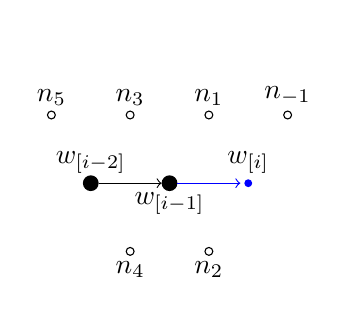
\begin{tikzpicture}
      \draw[white] (60:2) circle [radius=0.05];
      \node[right, white] at (60:2) {$n_{adj}$};
      
      \fill[shift=(180:1)] (0,0) circle [radius=0.1];
      \fill[shift=(180:0)] (0,0) circle [radius=0.1];
      
      \fill[blue](0:1) circle [radius=0.05];
      
      \draw[->] (180:0.9) -- (180:0.1);
      \draw[->, blue] (0:0.1) -- (0:0.9);

	\node[above] at (180:1) {$w_{[i-2]}$};
	\node[below] at (180:0) {$w_{[i-1]}$};
	\node[above] at (0:1) {$w_{[i]}$};

	\foreach \theta in {60,-60,120,-120}{
   	   \draw [shift=(\theta:1)] (0:0) circle [radius=0.05];
  	}
	 \draw [shift=(60:1), ] (0:1) circle [radius=0.05];
	  \draw [shift=(180:1),shift=(120:1)] (0:0) circle [radius=0.05];
 	\node[above] at (60:1) {$n_1$};
	\node[below] at (-60:1) {$n_2$};
	\node[above] at (120:1) {$n_3$};
	\node[below] at (-120:1) {$n_4$};
	\node[above, shift=(0:1)] at (60:1) {$n_{-1}$};
	\node[above, shift=(180:1)] at (120:1) {$n_5$};
    \end{tikzpicture}
    \end{minipage}
    
    \begin{minipage}{0.3\hsize}
    \centering
     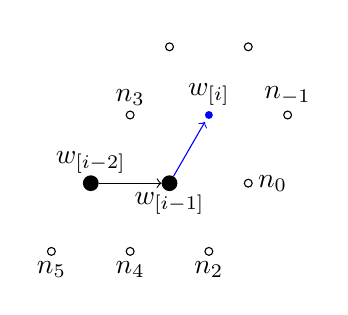
\begin{tikzpicture}
	\node[right, shift=(60:1), white] at (60:1) {$n_{adj}$};
      \fill[shift=(180:1)] (0,0) circle [radius=0.1];
      \fill[shift=(180:0)] (0,0) circle [radius=0.1];
      
      \fill[blue](60:1) circle [radius=0.05];
      
      \draw[->] (180:0.9) -- (180:0.1);
      \draw[->, blue] (60:0.1) -- (60:0.9);

	\node[above] at (180:1) {$w_{[i-2]}$};
	\node[below] at (180:0) {$w_{[i-1]}$};
	\node[above] at (60:1) {$w_{[i]}$};


	\foreach \theta in {0,-60,120,-120}{
   	   \draw [shift=(\theta:1)](0:0) circle [radius=0.05];
  	}
	\draw [shift=(60:1)] (0:1) circle [radius=0.05];
	\draw [shift=(60:1), shift=(60:1)] (0:0) circle [radius=0.05];
	\draw [shift=(60:1), shift=(120:1)] (0:0) circle [radius=0.05];
	  \draw [shift=(180:1),shift=(-120:1)] (0:0) circle [radius=0.05];
	
 	\node[right] at (0:1) {$n_0$};
	\node[below] at (-60:1) {$n_2$};
	\node[above] at (120:1) {$n_3$};
	\node[below] at (-120:1) {$n_4$};
	\node[above, shift=(60:1)] at (0:1) {$n_{-1}$};
	\node[below, shift=(180:1)] at (-120:1) {$n_5$};
    \end{tikzpicture}
    \end{minipage}
    
    \begin{minipage}{0.3\hsize}
        \centering
     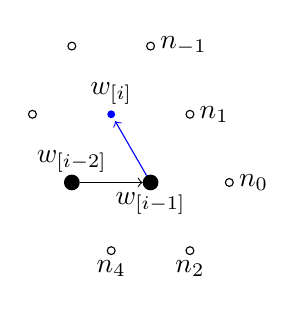
\begin{tikzpicture}
      
      \fill[shift=(180:1)] (0,0) circle [radius=0.1];
      \fill[shift=(180:0)] (0,0) circle [radius=0.1];
      
      \fill[blue](120:1) circle [radius=0.05];
      
      \draw[->] (180:0.9) -- (180:0.1);
      \draw[->, blue] (120:0.1) -- (120:0.9);

	\node[above] at (180:1) {$w_{[i-2]}$};
	\node[below] at (180:0) {$w_{[i-1]}$};
	\node[above] at (120:1) {$w_{[i]}$};


	\foreach \theta in {0,60,-60,-120}{
   	   \draw [shift=(\theta:1)] (0:0) circle [radius=0.05];
  	}
	\draw [shift=(120:1), shift=(60:1)] (0:0) circle [radius=0.05];
	\draw [shift=(120:1), shift=(120:1)] (0:0) circle [radius=0.05];
	\draw [shift=(120:1), shift=(180:1)] (0:0) circle [radius=0.05];
	
 	\node[right] at (0:1) {$n_0$};
	\node[right] at (60:1) {$n_1$};
	\node[below] at (-60:1) {$n_2$};
	\node[below] at (-120:1) {$n_4$};
	\node[right, shift=(120:1)] at (60:1) {$n_{-1}$};
    \end{tikzpicture}
    \end{minipage}
    \end{tabular}
    \caption{All possible directions of $w[i]$: straight, obtuse, acute.}
    \label{TTT_a3_w}
  \end{center}
\end{figure}




\begin{figure}[tb]
  \begin{center}
  \begin{tabular}{c c}
  \begin{minipage}{0.48\hsize}
  \centering
    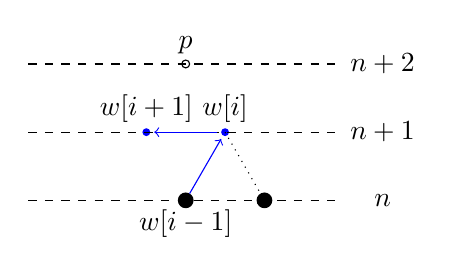
\begin{tikzpicture}
      	\fill (0,0) circle [radius=0.1];
        \fill[blue] (60:1) circle [radius=0.05];
         \fill[blue] (120:1) circle [radius=0.05];
        \fill (0:1) circle [radius=0.1];
      
      \draw[dashed] (180:2) -- (0:2);
      \draw[dashed, shift=(60:1)] (180:2.5) -- (0:1.5);
       \draw[dashed, shift=(60:2)] (180:3) -- (0:1);
      \draw[->, blue] (60:0.1) -- (60:0.9);
      \draw[->, blue, shift=(60:1)] (180:0.1) -- (180:0.9);
      
      \draw[dotted, shift = (60:1)] (0:0) -- (-60:1);
      

	\node[above,shift=(120:1)]at (60:1) {$p$};

	\draw[shift=(120:1)] (60:1) circle [radius=0.05];

	\node at (0:2.5) {$n$};
	\node[shift=(60:1)] at (0:2) {$n+1$};
	\node[shift=(60:2)] at (0:1.5) {$n+2$};
	
	\node[below] at (0:0) {$w[i-1]$};
	\node[above] at (60:1) {$w[i]$};
	\node[above] at (120:1) {$w[i+1]$};
	\end{tikzpicture}
    \end{minipage}
    
    \begin{minipage}{0.48\hsize}
    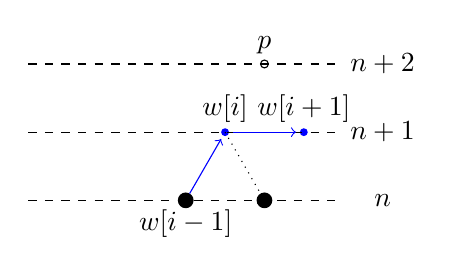
\begin{tikzpicture}
      	\fill (0,0) circle [radius=0.1];
        \fill[blue] (60:1) circle [radius=0.05];
         \fill[blue,shift=(0:1)] (60:1) circle [radius=0.05];
        \fill (0:1) circle [radius=0.1];
      
      \draw[dashed] (180:2) -- (0:2);
      \draw[dashed, shift=(60:1)] (180:2.5) -- (0:1.5);
       \draw[dashed, shift=(60:2)] (180:3) -- (0:1);
      \draw[->, blue] (60:0.1) -- (60:0.9);
      \draw[->, blue, shift=(60:1)] (0:0.1) -- (0:0.9);
       \draw[dotted, shift = (60:1)] (0:0) -- (-60:1);
      

	\node[above] at (60:2) {$p$};

	\draw (60:2) circle [radius=0.05];

	\node at (0:2.5) {$n$};
	\node[shift=(60:1)] at (0:2) {$n+1$};
	\node[shift=(60:2)] at (0:1.5) {$n+2$};
	
	\node[below] at (0:0) {$w[i-1]$};
	\node[above] at (60:1) {$w[i]$};
	\node[above, shift=(0:1)] at (60:1) {$w[i+1]$};
	\end{tikzpicture}
    \end{minipage}
    \end{tabular}
    \caption{The moment when the transcript steps outside $\hexagon^n_O$.}
    \label{fig:ttt_d2}
  \end{center}
\end{figure}



\begin{theorem}[$\delta= 1, \alpha=2$]
Let $\Xi$ be a deterministic unary oritatami system of $\delta = 1, \alpha = 2$.
It can yield an infinite structure, but the transcript folds into the zig-zag conformation after its $(27n^2 + 9n +1)$-th bead.
\end{theorem}

\begin{proof}
 We assume $w[i]$ is the first bead stabilized outside $\hexagon^n_O$.
 See Fig.~\ref{fig:ttt_d2}.
 The next bead $w[i+1]$ is to be bound for stabilization.
 Hence, it goes to the west  or to the east (Fig.~\ref{fig:ttt_d2}).
 Once $w[i+2]$ is stabilized at $p$, the remaining transcript folds into the zig-zag conformation.
 In order to avoid this or nondeterminism, $w[i+2]$ must form two bonds; it thus decreases binding capability by 1.
 Until when a bead is stabilized outside $\hexagon^{n+1}_O$, binding capability never increases because of arity being 2 and of the Tunnel Troll Theorem.
 This means that, only at most $\#bc(C_0) \leq 2n$ times we can thus expand that hexagonal region.
 In other words, outside $\hexagon^{3n}_O$ the transcript cannot help but fold zig-zag. \qed
 
\end{proof}



\subsection{Quadratic upper bounds for arity 1 and delay 2 or 3}
\label{sec:unary}

In this section we will argue that unary systems at arity $1$ and delay $2$ and $3$, respectively, cannot fold infinite transcripts deterministically. As we will see, in fact, the length of transcripts deterministically foldable by these systems has an upper bound quadratic in the length $n$ of the seed. The main result is the following theorem, which is a direct consequence of Lemmas~\ref{lem:d2a1}  and \ref{lem:d3a1} which follow.
\begin{theorem}[$\delta\in\{ 2,3\}, \alpha = 1$]\label{thm:d23a1}
	The terminal conformation of a deterministic unary oritatami system at arity $\alpha = 1$ and delay $\delta \in \{2,3\}$ is of length at most $3n^2+4n+2$.
\end{theorem}

%\begin{figure}
\begin{wrapfigure}{r}{0.5\linewidth}
	\centering
	\includegraphics[width=0.45\linewidth]{./Fig/hexagonOut}
	\caption{$\hexagon_p^n$ and the position $(1,1)$ of the first bead fixed outside of it.}
	\label{fig:hexagonOut}
\end{wrapfigure}
%\end{figure}

Let us fix some common starting points for Lemmas~\ref{lem:d2a1} and \ref{lem:d3a1}. Let the point where the first transcript bead was fixed be $p$. We will argue about the situation when the first bead is stabilized outside $\hexagon_p^n$ (a hexagon of radius $n$). Let this be the $i$th bead of the transcript. Without loss of generality, we can translate the origin $(0,0)$ to the coordinates of bead $i-1$ (which is still in $\hexagon_p^n$), and we can assume that bead $i$ is fixed at $(1,1)$ (see Fig.~\ref{fig:hexagonOut}).

%\subsubsection{\ref{sec:unary}.1 \ \ $\delta = 2$\\}
\begin{lemma}[$\delta=2, \alpha =1$]\label{lem:d2a1}
	The terminal conformation of a deterministic unary oritatami system of $\delta=2$ and $\alpha = 1$ is of length at most $3n^2+4n+2$.
\end{lemma}
\begin{proof}
In the elongation that places bead $i$ at $(1,1)$ there are two possibilities. 
\begin{itemize}
	\item $i$ forms a bond with a bead at $(1,0)$.
	\item  $i$ does not bond to anything and $i+1$ is at $(2,1)$ bonding with a bead at $(2,0)$. If there is no bead at $(1,0)$, then placing $i$ at $(1,0)$ instead of $(1,1)$ results in the same number of bonds, leading to nondeterminism. Therefore, there has to be a bead at $(1,0)$ and it is inactive, otherwise it would bond to $i$. This is analogous to case 1. below, with the only difference being that the bond between (1,1) and (1,0) is missing.%as in Fig.~\ref{fig:hexagonOut1}.
\end{itemize}

	\begin{figure}
		\centering
		\includegraphics[width=0.2\linewidth]{./Fig/hexagonOut1}
		%\caption{}
		\label{fig:hexagonOut1}
	\end{figure}
 
%The only position with which $(1,1)$ can form a bond is $(1,0)$. This means that there is a bead at $(1,0)$, which bonds to bead $i$, otherwise there are other conformations in which beads $i$ and $i+1$ add one bond to the conformation, making the behavior nondeterministic.
Because of the above, we need only consider the case when $i$ binds to a bead at (1,0). The next bead, $i+1$, can be fixed at $(2,1)$ or at $(0,1)$ as all other possibilities result in nondeterministic behavior immediately, so we have two cases.

%\begin{enumerate}
\noindent\textbf{Case 1.} bead $i+1$ is fixed at $(2,1)$ and can bond with a bead at $(2,0)$ (see Fig.~\ref{fig:hexagonOut2}). Now consider bead $i+2$. For $i+1$ to be fixed at $(2,1)$, $i+2$ needs to form a bond somewhere, otherwise $i+2$ could go to $(2,1)$ forming the bond with the bead at $(2,0)$ and there would be two conformations with the maximal $1$ bond. The only possibility is that there is a bead at $(3,0)$ and $i+2$ can bond with it when placed at $(3,1)$. We can apply the same argument inductively: there is some $m\geq 0$ such that grid points $(\ell,0)$ are occupied by beads with free hands, for all $\ell\in \{2,\dots,2+m\}$, and there is no bead at $(3+m,0)$. Such an $m$ exists, and it is not greater than $n$, because those beads are all stabilized along the same side of $\hexagon_p^n$. Then, bead $i+\ell$ is fixed at $(\ell+1,1)$ and bonds with $(\ell+1,0)$. However, bead $i+2+m$ cannot be fixed anywhere, because $i+2+m$ and $i+3+m$ can only add one bond to the conformation, and that is possible either with $i+2+m \rightarrow (2+m,1)$, $i+3+m \rightarrow (3+m,1)$ or with $i+2+m \rightarrow (2+m,2)$, $i+3+m \rightarrow (2+m,1)$. Intuitively, when we reach a corner of the hexagon $\hexagon_p^n$, the next bead of the transcript cannot deterministically stabilize, as depicted in Fig.~\ref{fig:hexagonOut2}. In this case, the size of the transcript which was deterministically stabilized is bounded by the size of $\hexagon_p^n$ plus the length of one side of $\hexagon_p^{n+1}$, so by $(3n^2+3n+1)+(n+1)=3n^2+4n+2$.
	\begin{figure}[h]
		\centering
		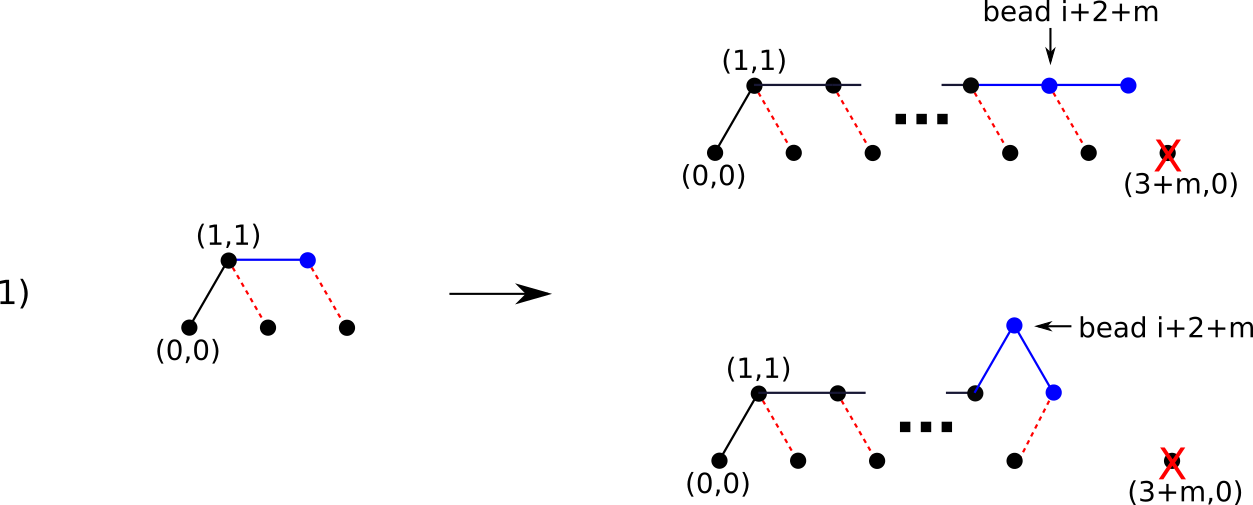
\includegraphics[width=0.9\linewidth]{./Fig/hexagonOut2}
		\caption{When bead $i+2+m$ is fixed}
		\label{fig:hexagonOut2}
	\end{figure}

\vspace{0.2cm}
	
\noindent\textbf{Case 2.} bead $i+1$ is fixed at $(0,1)$. This is only possible if\\
\textbf{(a)} there is an inactive bead at $(-1,0)$ and one with a free hand one at $(-2,0)$. This case is symmetrical to (1).
there is no bead at $(-1,0)$, bead $i+1$ can bond with bead $i-1$ at $(0,0)$ and the bead $i+2$ can be placed at $(-1,0)$ where it can bond with $(-2,0)$, $(-2,-1)$ or $(-1,-1)$. This leads to nondeterminism, because placing bead $i$ at $(-1,0)$ and bead $i+1$ at $(0,1)$ would yield two bonds, just as the original conformation.\\
\textbf{(b)	} there is a bead at $(-1,0)$ and bead $i+1$ can bond with that or with bead $i-1$ at $(0,0)$. However, this means that placing bead $i$ at $(0,1)$ at bead $i+1$ at $(1,1)$ creates the same number of hydrogen bonds, thus resulting in bead $i$ not being placed deterministically.
		
%\end{enumerate}




\begin{figure}[tb]
	\centering
	%\includegraphics[width=0.3\linewidth]{./hexagonOut1}
	%\hspace{10mm} %
	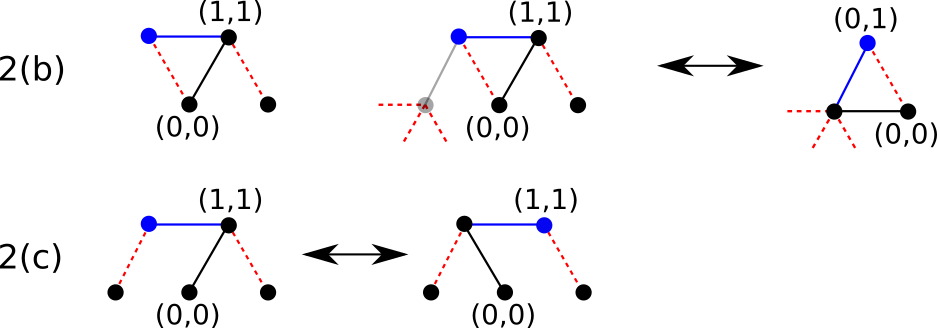
\includegraphics[width=0.8\linewidth]{./Fig/hexagonOut3n}
	
	\caption{When bead $i+1$ is fixed at (0,1)}
	\label{fig:hexagonOut3}
\end{figure}

Case 2.(a) gives the same upper bound as case 1. Cases 2.(b)-(c) give the smaller upper bound $|\hexagon_p^n|+1$, thereby concluding the proof.
\qed
\end{proof}

%\subsubsection{\ref{sec:unary}.2 \ \ $\delta = 3$\\}

\begin{lemma}[$\delta=3, \alpha =1$]\label{lem:d3a1}
	The terminal conformation of a deterministic unary oritatami system of $\delta=3$ and $\alpha = 1$ is of length at most $3n^2+4n+2$.
\end{lemma}
\begin{proof}
We will argue similarly to the $\delta=2$ case: when we stabilize beads outside $\hexagon_p^n$, we can only do so at points right next to one of the sides and even there only until we reach a corner. This yields the upper bound immediately.

As before, let us assume that the last bead stabilized within $\hexagon_p^n$ is at point $(0,0)$ and the next bead is the first to be stabilized outside $\hexagon_p^n$ at point $(1,1)$. Depending on whether bead $i-1$ at point (0,0) has a free hand to form a bond or not, we distinguish two cases.\\
%\begin{enumerate}
\noindent\textbf{Case 1.}  Bead $i-1$ at (0,0) has a free hand. If the most stable conformation formed by beads $i, i+1, i+2$ adds only two  bonds, it will be nondeterministic because there are at least two possibilities (see Fig.~\ref{fig:beadi2}, except it starts from (0,0) not (1,1)). Therefore, it needs to make three new bonds to deterministically stabilize $i$. There are five possible cases in which beads $i, i+1, i+2$ can add three bonds, see Fig.~\ref{fig:3bonds}. In the cases (b) and (e) in Fig.~\ref{fig:3bonds}, there are beads having a free hand at (1,0) and (-1,0) already stabilized before bead $i-1$ is fixed at (0,0). One of these two beads may be a predecessor of bead $i-1$, but at least one of them is not. When bead $i-1$ is fixed at (0,0), it makes a bond with the one of these two beads which is not its predecessor. This means that it is impossible to have three beads at (-1,0), (0,0) and (1,0), each with a free hand, when bead $i$ is fixed, and consequently, cases (b) and (e) in Fig.~\ref{fig:3bonds} cannot occur. Case (d) in Fig.~\ref{fig:3bonds} becomes nondeterministic when bead $i$ is fixed because bead $i$ can be fixed at (-1,0) and bond with (-2,0), bead $i+1$ can be placed (0,1) and bond with (0,0) and bead $i+2$ can be placed (1,1) and bond with (0,1). If it makes three bonds once, such as (a) and (c) in Fig.~\ref{fig:3bonds}, it will need to make three bonds forever to be deterministic. Similarly to case 1. in the previous section, cases (a) and (c) in Fig.~\ref{fig:3bonds} lead to nondeterministism eventually, when the transcript reaches a first corner of $\hexagon_p^n$.

\begin{figure}
	\begin{center}
		\begin{tabular}{ccccc}
			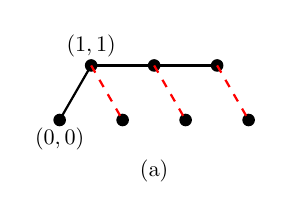
\begin{tikzpicture}[thick,scale=0.8, every node/.style={scale=0.8}]
			\fill (0.0, 0.0) circle [radius = 0.1];
			\fill (1.0, 0.0) circle [radius = 0.1];
			\fill (2.0, 0.0) circle [radius = 0.1];
			\fill (3.0, 0.0) circle [radius = 0.1];
			\fill (0.5, 0.866) circle [radius = 0.1];
			\fill (1.5, 0.866) circle [radius = 0.1];
			\fill (2.5, 0.866) circle [radius = 0.1];
			\fill (0.0, 0.0) node [below] {$(0, 0)$};
			\fill (0.5, 0.866) node [above] {$(1, 1)$};
			\draw (0.0, 0.0) -- (0.5, 0.866);
			\draw (0.5, 0.866) -- (1.5, 0.866);
			\draw (1.5, 0.866) -- (2.5, 0.866);
			\draw [dashed] [red] (0.5, 0.866) -- (1.0, 0.0);
			\draw [dashed] [red] (1.5, 0.866) -- (2.0, 0.0);
			\draw [dashed] [red] (2.5, 0.866) -- (3.0, 0.0);
			\fill (1.5, -0.5) node [below] {(a)};
			\end{tikzpicture}
			
			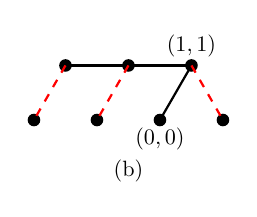
\begin{tikzpicture}[thick,scale=0.8, every node/.style={scale=0.8}]
			\fill (1.0, 0.0) circle [radius = 0.1];
			\fill (0.0, 0.0) circle [radius = 0.1];
			\fill (-1.0, 0.0) circle [radius = 0.1];
			\fill (-2.0, 0.0) circle [radius = 0.1];
			\fill (0.5, 0.866) circle [radius = 0.1];
			\fill (-0.5, 0.866) circle [radius = 0.1];
			\fill (-1.5, 0.866) circle [radius = 0.1];
			\fill (0.0, 0.0) node [below] {$(0, 0)$};
			\fill (0.5, 0.866) node [above] {$(1, 1)$};
			\draw (0.0, 0.0) -- (0.5, 0.866);
			\draw (0.5, 0.866) -- (-0.5, 0.866);
			\draw (-0.5, 0.866) -- (-1.5, 0.866);
			\draw [dashed] [red] (0.5, 0.866) -- (1.0, 0.0);
			\draw [dashed] [red] (-0.5, 0.866) -- (-1.0, 0.0);
			\draw [dashed] [red] (-1.5, 0.866) -- (-2.0, 0.0);
			\fill (-0.5, -0.5) node [below] {(b)};
			\end{tikzpicture}
			
			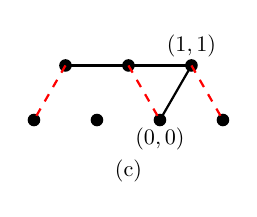
\begin{tikzpicture}[thick,scale=0.8, every node/.style={scale=0.8}]
			\fill (1.0, 0.0) circle [radius = 0.1];
			\fill (0.0, 0.0) circle [radius = 0.1];
			\fill (-1.0, 0.0) circle [radius = 0.1];
			\fill (-2.0, 0.0) circle [radius = 0.1];
			\fill (0.5, 0.866) circle [radius = 0.1];
			\fill (-0.5, 0.866) circle [radius = 0.1];
			\fill (-1.5, 0.866) circle [radius = 0.1];
			\fill (0.0, 0.0) node [below] {$(0, 0)$};
			\fill (0.5, 0.866) node [above] {$(1, 1)$};
			\draw (0.0, 0.0) -- (0.5, 0.866);
			\draw (0.5, 0.866) -- (-0.5, 0.866);
			\draw (-0.5, 0.866) -- (-1.5, 0.866);
			\draw [dashed] [red] (0.5, 0.866) -- (1.0, 0.0);
			\draw [dashed] [red] (-0.5, 0.866) -- (0.0, 0.0);
			\draw [dashed] [red] (-1.5, 0.866) -- (-2.0, 0.0);
			\fill (-0.5, -0.5) node [below] {(c)};
			\end{tikzpicture}
			
			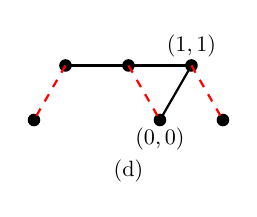
\begin{tikzpicture}[thick,scale=0.8, every node/.style={scale=0.8}]
			\fill (1.0, 0.0) circle [radius = 0.1];
			\fill (0.0, 0.0) circle [radius = 0.1];
			\fill (-2.0, 0.0) circle [radius = 0.1];
			\fill (0.5, 0.866) circle [radius = 0.1];
			\fill (-0.5, 0.866) circle [radius = 0.1];
			\fill (-1.5, 0.866) circle [radius = 0.1];
			\fill (0.0, 0.0) node [below] {$(0, 0)$};
			\fill (0.5, 0.866) node [above] {$(1, 1)$};
			\draw (0.0, 0.0) -- (0.5, 0.866);
			\draw (0.5, 0.866) -- (-0.5, 0.866);
			\draw (-0.5, 0.866) -- (-1.5, 0.866);
			\draw [dashed] [red] (0.5, 0.866) -- (1.0, 0.0);
			\draw [dashed] [red] (-0.5, 0.866) -- (0.0, 0.0);
			\draw [dashed] [red] (-1.5, 0.866) -- (-2.0, 0.0);
			\fill (-0.5, -0.5) node [below] {(d)};
			\end{tikzpicture}
			
			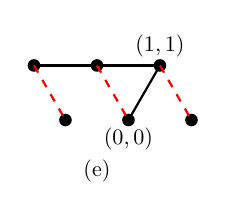
\begin{tikzpicture}[thick,scale=0.8, every node/.style={scale=0.8}]
			\fill (1.0, 0.0) circle [radius = 0.1];
			\fill (0.0, 0.0) circle [radius = 0.1];
			\fill (-1.0, 0.0) circle [radius = 0.1];
			\fill (0.5, 0.866) circle [radius = 0.1];
			\fill (-0.5, 0.866) circle [radius = 0.1];
			\fill (-1.5, 0.866) circle [radius = 0.1];
			\fill (0.0, 0.0) node [below] {$(0, 0)$};
			\fill (0.5, 0.866) node [above] {$(1, 1)$};
			\draw (0.0, 0.0) -- (0.5, 0.866);
			\draw (0.5, 0.866) -- (-0.5, 0.866);
			\draw (-0.5, 0.866) -- (-1.5, 0.866);
			\draw [dashed] [red] (0.5, 0.866) -- (1.0, 0.0);
			\draw [dashed] [red] (-0.5, 0.866) -- (0.0, 0.0);
			\draw [dashed] [red] (-1.5, 0.866) -- (-1.0, 0.0);
			\fill (-0.5, -0.5) node [below] {(e)};
			\end{tikzpicture}\\
			
		\end{tabular}
		\caption{When beads $i, i+1, i+2$ make three hydrogen bonds (c) there is an inactive bead at (-1,0).  (d) there is no bead at (-1,0).}
		\label{fig:3bonds}
	\end{center}
\end{figure}

\noindent\textbf{Case 2.} Bead $i-1$ at (0,0) does not have a free hand.\\
(i) First, let us assume that there is a bead at (1,0) which has a free hand. If there is a bead at (1,0) and beads $i, i+1, i+2$ add only two bonds, we instantly get nondeterministism as in Fig.~\ref{fig:beadat(1,0)}. Hence, beads $i, i+1, i+2$ need to make three bonds to stabilize $i$, but if they make three hydrogen bonds, the situation is analogous to (a) and (c) in Fig.~\ref{fig:3bonds}. 

%There are not any bead having a free hand at (1,0) or (-1,0) to prevent from being (a) and (c) in Fig.~\ref{fig:3bonds}. 
\noindent (ii) Now consider when there is no bead at (1,0) or there is one, but with no free hand. Let us discuss the moment after bead $i$ is fixed outside $\hexagon_p^n$. Now bead $i$ has a free hand because it cannot bind to (1,0). If beads $i+1, i+2, i+3$ can form only two bonds, it will be nondeterministic because there are at least two possible such conformations, as in Fig.~\ref{fig:beadi2}. Hence, they need to form three bonds to deterministically stabilize, such as in Fig.~\ref{fig:3bonds2}. Case (a) in Fig.~\ref{fig:3bonds2}. becomes the same as case (a) in Fig.~\ref{fig:3bonds}. Case (b) in Fig.~\ref{fig:3bonds2} becomes nondeterministic already when bead $i$ is fixed because bead $i$ could also be fixed at (1,0).\\

\begin{figure}
	\begin{minipage}{.45\textwidth}
		
	
  \begin{center}
    \begin{tabular}{cc}
      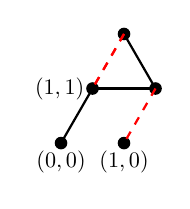
\begin{tikzpicture}[thick,scale=0.8, every node/.style={scale=0.8}]
        \fill (0.0, 0.0) circle [radius = 0.1];
        \fill (1.0, 0.0) circle [radius = 0.1];
        \fill (0.5, 0.866) circle [radius = 0.1];
        \fill (1.5, 0.866) circle [radius = 0.1];
        \fill (1.0, 1.732) circle [radius = 0.1];
        \fill (0.0, 0.0) node [below] {$(0, 0)$};
        \fill (0.5, 0.866) node [left] {$(1, 1)$};
        \fill (1.0, 0.0) node [below] {$(1, 0)$};
        \draw (0.0, 0.0) -- (0.5, 0.866);
        \draw (0.5, 0.866) -- (1.5, 0.866);
        \draw (1.0, 1.732) -- (1.5, 0.866);
        \draw [dashed] [red] (1.5, 0.866) -- (1.0, 0.0);
        \draw [dashed] [red] (1.0, 1.732) -- (0.5, 0.866);
        \draw [dashed] [red] (1.0, 1.732) -- (0.5, 0.866);
      \end{tikzpicture}

      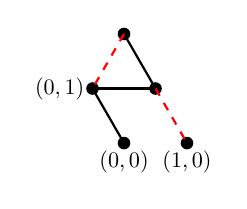
\begin{tikzpicture}[thick,scale=0.8, every node/.style={scale=0.8}]
        \fill (0.0, 0.0) circle [radius = 0.1];
        \fill (1.0, 0.0) circle [radius = 0.1];
        \fill (-0.5, 0.866) circle [radius = 0.1];
        \fill (0.5, 0.866) circle [radius = 0.1];
        \fill (0.0, 1.732) circle [radius = 0.1];
        \fill (0.0, 0.0) node [below] {$(0, 0)$};
        \fill (-0.5, 0.866) node [left] {$(0, 1)$};
        \fill (1.0, 0.0) node [below] {$(1, 0)$};
        \draw (0.0, 0.0) -- (-0.5, 0.866);
        \draw (-0.5, 0.866) -- (0.5, 0.866);
        \draw (0.0, 1.732) -- (0.5, 0.866);
        \draw [dashed] [red] (0.5, 0.866) -- (1.0, 0.0);
        \draw [dashed] [red] (0.0, 1.732) -- (-0.5, 0.866);
      \end{tikzpicture}

    \end{tabular}
    \caption{Two conformations when a bead at (1,0) has a free hand.}
    \label{fig:beadat(1,0)}
  \end{center}
	\end{minipage}%	
\hspace{1cm}\begin{minipage}{.45\textwidth}
		\begin{center}
			\begin{tabular}{cc}
				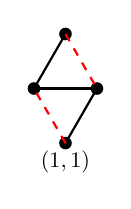
\begin{tikzpicture}[thick,scale=0.8, every node/.style={scale=0.8}]
				\fill (0.0, 0.0) circle [radius = 0.1];
				\fill (0.5, 0.866) circle [radius = 0.1];
				\fill (-0.5, 0.866) circle [radius = 0.1];
				\fill (0.0, 1.732) circle [radius = 0.1];
				\fill (0.0, 0.0) node [below] {$(1, 1)$};
				\draw (0.0, 0.0) -- (0.5, 0.866);
				\draw (0.5, 0.866) -- (-0.5, 0.866);
				\draw (0.0, 1.732) -- (-0.5, 0.866);
				\draw [dashed] [red] (0.0, 1.732) -- (0.5, 0.866);
				\draw [dashed] [red] (0.0, 0.0) -- (-0.5, 0.866);
				\end{tikzpicture}
				
				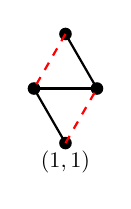
\begin{tikzpicture}[thick,scale=0.8, every node/.style={scale=0.8}]
				\fill (0.0, 0.0) circle [radius = 0.1];
				\fill (-0.5, 0.866) circle [radius = 0.1];
				\fill (0.5, 0.866) circle [radius = 0.1];
				\fill (0.0, 1.732) circle [radius = 0.1];
				\fill (0.0, 0.0) node [below] {$(1, 1)$};
				\draw (0.0, 0.0) -- (-0.5, 0.866);
				\draw (-0.5, 0.866) -- (0.5, 0.866);
				\draw (0.0, 1.732) -- (0.5, 0.866);
				\draw [dashed] [red] (0.0, 0.0) -- (0.5, 0.866);
				\draw [dashed] [red] (0.0, 1.732) -- (-0.5, 0.866);
				\end{tikzpicture}
				
			\end{tabular}
			\caption{Two conformations when a bead $i$ at (1,1) has a free hand}
			\label{fig:beadi2}
		\end{center}
	\end{minipage}

\end{figure}


%
%\begin{figure}
%  \begin{center}
%    \begin{tabular}{cc}
%      \begin{tikzpicture}[thick,scale=0.8, every node/.style={scale=0.8}]
%        \fill (0.0, 0.0) circle [radius = 0.1];
%        \fill (0.5, 0.866) circle [radius = 0.1];
%        \fill (-0.5, 0.866) circle [radius = 0.1];
%        \fill (0.0, 1.732) circle [radius = 0.1];
%        \fill (0.0, 0.0) node [below] {$(1, 1)$};
%        \draw (0.0, 0.0) -- (0.5, 0.866);
%        \draw (0.5, 0.866) -- (-0.5, 0.866);
%        \draw (0.0, 1.732) -- (-0.5, 0.866);
%        \draw [dashed] [red] (0.0, 1.732) -- (0.5, 0.866);
%        \draw [dashed] [red] (0.0, 0.0) -- (-0.5, 0.866);
%      \end{tikzpicture}
%
%      \begin{tikzpicture}[thick,scale=0.8, every node/.style={scale=0.8}]
%        \fill (0.0, 0.0) circle [radius = 0.1];
%        \fill (-0.5, 0.866) circle [radius = 0.1];
%        \fill (0.5, 0.866) circle [radius = 0.1];
%        \fill (0.0, 1.732) circle [radius = 0.1];
%        \fill (0.0, 0.0) node [below] {$(1, 1)$};
%        \draw (0.0, 0.0) -- (-0.5, 0.866);
%        \draw (-0.5, 0.866) -- (0.5, 0.866);
%        \draw (0.0, 1.732) -- (0.5, 0.866);
%        \draw [dashed] [red] (0.0, 0.0) -- (0.5, 0.866);
%        \draw [dashed] [red] (0.0, 1.732) -- (-0.5, 0.866);
%      \end{tikzpicture}
%
%    \end{tabular}
%    \caption{Two conformations when a bead $i$ at (1,1) has a free hand}
%    \label{fig:beadi2}
%  \end{center}
%\end{figure}



\begin{figure}
  \begin{center}
    \begin{tabular}{cc}

      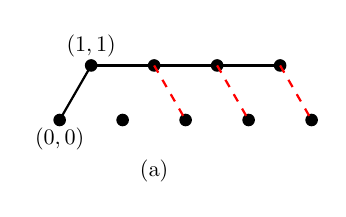
\begin{tikzpicture}[thick,scale=0.8, every node/.style={scale=0.8}]
        \fill (0.0, 0.0) circle [radius = 0.1];
        \fill (1.0, 0.0) circle [radius = 0.1];
        \fill (2.0, 0.0) circle [radius = 0.1];
        \fill (3.0, 0.0) circle [radius = 0.1];
        \fill (4.0, 0.0) circle [radius = 0.1];
        \fill (0.5, 0.866) circle [radius = 0.1];
        \fill (1.5, 0.866) circle [radius = 0.1];
        \fill (2.5, 0.866) circle [radius = 0.1];
        \fill (3.5, 0.866) circle [radius = 0.1];
        \fill (0.0, 0.0) node [below] {$(0, 0)$};
        \fill (0.5, 0.866) node [above] {$(1, 1)$};
        \draw (0.0, 0.0) -- (0.5, 0.866);
        \draw (0.5, 0.866) -- (1.5, 0.866);
        \draw (1.5, 0.866) -- (2.5, 0.866);
        \draw (2.5, 0.866) -- (3.5, 0.866);
        \draw [dashed] [red] (1.5, 0.866) -- (2.0, 0.0);
        \draw [dashed] [red] (2.5, 0.866) -- (3.0, 0.0);
        \draw [dashed] [red] (3.5, 0.866) -- (4.0, 0.0);
        \fill (1.5, -0.5) node [below] {(a)};
      \end{tikzpicture}
      
      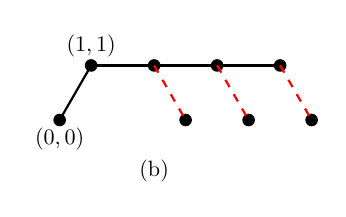
\begin{tikzpicture}[thick,scale=0.8, every node/.style={scale=0.8}]
        \fill (0.0, 0.0) circle [radius = 0.1];
        \fill (2.0, 0.0) circle [radius = 0.1];
        \fill (3.0, 0.0) circle [radius = 0.1];
        \fill (4.0, 0.0) circle [radius = 0.1];
        \fill (0.5, 0.866) circle [radius = 0.1];
        \fill (1.5, 0.866) circle [radius = 0.1];
        \fill (2.5, 0.866) circle [radius = 0.1];
        \fill (3.5, 0.866) circle [radius = 0.1];
        \fill (0.0, 0.0) node [below] {$(0, 0)$};
        \fill (0.5, 0.866) node [above] {$(1, 1)$};
        \draw (0.0, 0.0) -- (0.5, 0.866);
        \draw (0.5, 0.866) -- (1.5, 0.866);
        \draw (1.5, 0.866) -- (2.5, 0.866);
        \draw (2.5, 0.866) -- (3.5, 0.866);
        \draw [dashed] [red] (1.5, 0.866) -- (2.0, 0.0);
        \draw [dashed] [red] (2.5, 0.866) -- (3.0, 0.0);
        \draw [dashed] [red] (3.5, 0.866) -- (4.0, 0.0);
        \fill (1.5, -0.5) node [below] {(b)};
      \end{tikzpicture}\\

    \end{tabular}
    \caption{When beads $i+1, i+2, i+3$ make three hydrogen bonds (a) there is an inactive bead at (1,0). (b) there is no bead at (1,0).}
    \label{fig:3bonds2}
  \end{center}
\end{figure}
We have shown that at $\alpha=1$ and  $\delta\in\{2,3\}$, unary oritatami systems can only fold finite length transcripts deterministically, and the length of that transcript is bounded by the size of the regular hexagon of radius $n$ plus the length of one side of the surrounding hexagon. This gives us the upper bound $|\hexagon_p^{n}|+(n+1)=3n^2+4n+2$,  where $n$ is the length of the seed, concluding the proof of Theorem~\ref{thm:d23a1}.
\end{proof}


\subsection*{Acknowledgements}
We thank Yo-Sub Han for his valuable comments on the contents of this paper. 

\bibliographystyle{splncs03}
\bibliography{tamc2019}
  
\end{document}
